% ============================================================
%  AXI-MM Based Cache Implementation — FYP Report
%  Ghulam Ishaq Khan Institute of Engineering Sciences and Technology
%  Faculty of Computer Engineering
% ============================================================
\documentclass[12pt,letterpaper]{report}

% ---- Packages -----------------------------------------------
\usepackage[top=1.5in,bottom=1.5in,left=2in,right=1.33in,
            headheight=15pt,headsep=0.3in]{geometry}
\usepackage{graphicx}
\usepackage{tikz}
\usepackage{pgfplots}
\pgfplotsset{compat=1.18}
\usetikzlibrary{shapes.geometric,arrows.meta,positioning,calc,
                fit,backgrounds,decorations.pathreplacing,matrix}
\usepackage{booktabs}
\usepackage{array}
\usepackage{multirow}
\usepackage{tabularx}
\usepackage{longtable}
\usepackage{listings}
\usepackage{xcolor}
\usepackage[hidelinks]{hyperref}
\usepackage{amsmath}
\usepackage{caption}
\usepackage{subcaption}
\usepackage{fancyhdr}
\usepackage{setspace}
\usepackage{tocloft}
\usepackage{titlesec}
\usepackage{enumitem}
\usepackage{mathptmx}
\usepackage[T1]{fontenc}
\usepackage{microtype}

% ---- Colours ------------------------------------------------
\definecolor{giki}{RGB}{0,51,102}
\definecolor{lightgray}{RGB}{245,245,245}
\definecolor{codegray}{RGB}{100,100,100}
\definecolor{codegreen}{RGB}{0,120,0}
\definecolor{codepurple}{RGB}{100,0,160}
\definecolor{covblue}{RGB}{41,128,185}
\definecolor{covorange}{RGB}{230,126,34}
\definecolor{covgreen}{RGB}{39,174,96}
\definecolor{covred}{RGB}{192,57,43}

% ---- Page style --------------------------------------------
\pagestyle{fancy}
\fancyhf{}
\fancyhead[L]{\small\nouppercase{\leftmark}}
\fancyhead[R]{\small\thepage}
\renewcommand{\headrulewidth}{0.4pt}
\setlength{\headheight}{15pt}
\setlength{\footskip}{0.5in}

% ---- Chapter / section formatting --------------------------
\titleformat{\chapter}[display]
  {\normalfont\fontsize{14}{17}\selectfont\bfseries\centering}
  {CHAPTER \Roman{chapter}}{4pt}
  {\normalfont\fontsize{14}{17}\selectfont\bfseries\centering}
\titlespacing*{\chapter}{0pt}{0pt}{18pt}

\titleformat{name=\chapter,numberless}
  {\normalfont\fontsize{14}{17}\selectfont\bfseries\centering}
  {}{0pt}{\MakeUppercase}
\titlespacing*{name=\chapter,numberless}{0pt}{0pt}{18pt}

\titleformat{\section}
  {\normalfont\fontsize{12}{15}\selectfont\bfseries}
  {\thesection}{1em}{}
\titlespacing*{\section}{0pt}{12pt}{6pt}

\titleformat{\subsection}
  {\normalfont\fontsize{12}{15}\selectfont\bfseries\itshape}
  {\thesubsection}{1em}{}
\titlespacing*{\subsection}{0pt}{10pt}{4pt}

% ---- Captions -----------------------------------------------
\captionsetup{font={footnotesize},labelfont={bf},justification=centering}

% ---- Listings style ----------------------------------------
\lstdefinestyle{sv}{
  language=Verilog,
  basicstyle=\ttfamily\small,
  keywordstyle=\color{giki}\bfseries,
  commentstyle=\color{codegreen}\itshape,
  stringstyle=\color{codepurple},
  numberstyle=\tiny\color{codegray},
  numbers=left, stepnumber=1, numbersep=6pt,
  frame=single, rulecolor=\color{gray!40},
  backgroundcolor=\color{lightgray},
  breaklines=true, tabsize=2,
  morekeywords={logic,always_ff,always_comb,posedge,negedge,
                parameter,localparam,module,endmodule,input,output,
                typedef,enum,unique,assign,begin,end,for,if,else,
                case,endcase,integer,int}
}

% ---- Spacing & justification --------------------------------
\onehalfspacing
\setlength{\parindent}{0.5in}

% ============================================================
\begin{document}

% ============================================================
%  TITLE PAGE
% ============================================================
\newgeometry{top=1.5in,bottom=0.39in,left=2in,right=1.33in}
\begin{titlepage}
\pagestyle{empty}
\centering
\vspace*{0pt}

\vspace{0.6cm}
{\fontsize{14}{17}\selectfont\bfseries
  Ghulam Ishaq Khan Institute of Engineering Sciences and Technology}\\[0.25cm]
{\fontsize{14}{17}\selectfont\bfseries Faculty of Computer Engineering}\\[0.2cm]
{\color{giki}\rule{\linewidth}{1pt}}\\[1.2cm]

{\fontsize{18}{22}\selectfont\bfseries
  AXI-MM Based Cache Implementation}\\[1.4cm]

{\fontsize{14}{18}\selectfont\bfseries
\begin{tabular}{@{}ll@{}}
  \textbf{Group Members:} & \\[4pt]
  M.\ Abdullah Saeed  & Reg.\ No.\ 2022329 \\[4pt]
  M.\ Abdullah Zafar  & Reg.\ No.\ 2022328 \\[4pt]
  Aqib Muhammad       & Reg.\ No.\ 2022103 \\[10pt]
  \textbf{Supervisor:}    & Dr.\ Waqar Ahmad       \\[4pt]
  \textbf{Co-Supervisor:} & Dr.\ Fahad Bin Muslim  \\[4pt]
  \textbf{Session:}   & 2025--2026         \\
\end{tabular}}\\[1.4cm]

{\color{giki}\rule{\linewidth}{1pt}}\\[0.5cm]
{\fontsize{14}{17}\selectfont\bfseries
  Faculty of Computer Engineering}\\[0.2cm]
{\fontsize{14}{17}\selectfont\bfseries
  Ghulam Ishaq Khan Institute of Engineering Sciences and Technology}\\[0.3cm]
{\large April 2026}
\end{titlepage}
\restoregeometry

% ============================================================
%  CERTIFICATE OF APPROVAL
% ============================================================
\clearpage
\pagestyle{empty}
\begin{center}
{\fontsize{14}{17}\selectfont\bfseries CERTIFICATE OF APPROVAL}
\end{center}
\vspace{18pt}

\noindent It is certified that the work presented in this Final Year Project
report, titled \textbf{``AXI-MM Based Cache Implementation,''} was
performed by \textbf{M.\ Abdullah Saeed (Reg.\ No.\ 2022329),
M.\ Abdullah Zafar (Reg.\ No.\ 2022328), and Aqib Muhammad
(Reg.\ No.\ 2022103)} under the supervision of
\textbf{Dr.\ Waqar Ahmad}, Faculty of Computer Engineering, Ghulam
Ishaq Khan Institute of Engineering Sciences and Technology.  The work
satisfies the requirements for the award of the degree of Bachelor of
Science in Computer Engineering and is approved for submission.

\vspace{2.5cm}

\noindent\begin{tabular}{@{}p{0.45\linewidth}p{0.45\linewidth}@{}}
\rule{0.40\linewidth}{0.4pt} & \rule{0.40\linewidth}{0.4pt} \\[2pt]
\textbf{Dr.\ Waqar Ahmad}   & \textbf{Dr.\ Fahad Bin Muslim} \\
Advisor                     & Co-Advisor \\
Faculty of Computer Engineering & Faculty of Computer Engineering \\
GIK Institute               & GIK Institute \\[2.5cm]
\end{tabular}

\noindent\begin{tabular}{@{}p{0.45\linewidth}@{}}
\rule{0.40\linewidth}{0.4pt} \\[2pt]
\textbf{Prof.\ Dr.\ Qadeer Ul Hassan} \\
Dean, Faculty of Computer Engineering \\
GIK Institute \\
\end{tabular}

\clearpage

% ============================================================
%  SDGs INCLUSION
% ============================================================
\begin{center}
{\fontsize{14}{17}\selectfont\bfseries SDGs INCLUSION}
\end{center}
\vspace{18pt}

\noindent This project aligns with the following United Nations Sustainable
Development Goals (SDGs):

\vspace{12pt}

\noindent\textbf{SDG 9 — Industry, Innovation and Infrastructure}\\[4pt]
The AXI-MM Based Cache subsystem directly supports Goal 9 by advancing
hardware infrastructure for high-performance, energy-efficient computing
systems.  Designing a formally verified, 4-way set-associative cache
with an AXI4-compliant interface and a non-blocking miss policy
demonstrates the application of modern engineering innovation to build
resilient and efficient digital infrastructure, which is a prerequisite
for industrial-grade embedded and SoC platforms.


\vspace{2.5cm}

\noindent\begin{tabular}{@{}p{0.45\linewidth}p{0.45\linewidth}@{}}
\rule{0.40\linewidth}{0.4pt} & \rule{0.40\linewidth}{0.4pt} \\[2pt]
\textbf{Dr.\ Waqar Ahmad}   & \textbf{Dr.\ Fahad Bin Muslim} \\
Advisor                     & Co-Advisor \\
\end{tabular}

\clearpage

% ============================================================
%  FRONT MATTER
% ============================================================
\pagestyle{fancy}
\pagenumbering{roman}

% ---- Abstract ----------------------------------------------
\chapter*{Abstract}
\addcontentsline{toc}{chapter}{Abstract}

This report presents the design and functional verification of an AXI4
memory-mapped 4-way set-associative cache subsystem implemented in
SystemVerilog.  The cache is 4\,KB in capacity, organised as 128 sets
of 4 ways with a 64-bit (8-byte) cache line.  It employs a
write-through, no-write-allocate policy with Pseudo-Least-Recently-Used
(PLRU) replacement and a 4-entry Miss Status Holding Register (MSHR) to
track outstanding memory fetches.  Write traffic is decoupled from the
CPU critical path through an 8-entry write buffer that drains to main
memory asynchronously.

The subsystem implements a \emph{non-blocking} miss policy: on a cold
read miss the arbiter dequeues the request immediately after MSHR
allocation, without stalling the request pipeline.  The cache continues
to serve subsequent requests while the memory fetch is outstanding.
Fill responses are delivered to the CPU through a depth-4 fill response
FIFO.  A separate \textsc{wait\_pending} state handles the narrower case
where a second request targets an address whose fill is already in
flight (a pending-hit stall), ensuring correct ordering without broader
pipeline blocking.

The entire subsystem---including tag store, status store, data store,
PLRU state store, hit detector, control FSM, MSHR, write buffer,
read/write FIFOs, round-robin arbiter, and a behavioural main-memory
model---is integrated in a single top-level AXI4 slave module.
Simulation was performed using Cadence Xcelium 25.03.  Ten directed
test cases covering cold misses, cache hits, write-through behaviour,
RAW forwarding, write hits, hit-under-miss, concurrent misses, and
pending-hit stall were executed; all 27 assertions passed with zero
failures.  Functional coverage collected via SystemVerilog covergroups
confirms 100\% exercise of fill-completion events, non-blocking miss
completions, and read/write $\times$ hit/miss cross-coverage.

\clearpage

% ---- Acknowledgements -------------------------------------
\chapter*{Acknowledgements}
\addcontentsline{toc}{chapter}{Acknowledgements}

The authors thank the Faculty of Computer Engineering at GIK Institute
for providing access to EDA tools and laboratory resources.  Special
thanks to Dr.\ Waqar Ahmad and Dr.\ Fahad Bin Muslim for their guidance
and technical mentorship throughout the project.  The authors also
acknowledge Cadence Design Systems for providing access to the Xcelium
Logic Simulator through the EDA Playground online platform.

\clearpage

% ---- Contents ---------------------------------------------
\tableofcontents
\clearpage
\listoffigures
\clearpage
\listoftables
\clearpage

% ============================================================
%  MAIN MATTER
% ============================================================
\pagenumbering{arabic}

% ============================================================
\chapter{Introduction}
% ============================================================

\section{Motivation}

Modern processors execute instructions several times faster than main
memory can supply operands.  Even a DDR5 DRAM with a raw bandwidth of
60\,GB/s imposes latencies of 60--80 clock cycles on a 3\,GHz
processor, creating a severe \emph{memory wall} that limits
instruction-level parallelism.  Cache memories---small, fast SRAM
structures that exploit spatial and temporal locality---bridge this gap
by serving the majority of memory references with single-cycle latency.

The memory wall problem is especially acute in pipelined and
out-of-order processors, where a single cache miss can drain the
instruction window and halt forward progress across multiple execution
units.  The classic solution is to combine a cache with a lockup-free
(non-blocking) miss policy: on a cache miss the pipeline is not
frozen; instead the miss is recorded in a Miss Status Holding Register
(MSHR) and execution continues.  If a subsequent request hits in the
cache, it is served normally.  If it targets the same in-flight line,
it is briefly stalled only until the fill arrives.  This
hit-under-miss capability converts long-latency memory stalls from
\emph{blocking} events into overlapped background activities.

As system-on-chip (SoC) designs increasingly adopt the Advanced
eXtensible Interface (AXI4) as the standard on-chip interconnect, a
cache that exposes an AXI4 slave interface becomes a first-class
building block compatible with any AXI4 master, from soft-core
processors to DMA engines.  This project designs, implements, and
verifies exactly such a component: a non-blocking, 4-way
set-associative cache subsystem with an AXI4 interface, fully
simulated and coverage-verified on Cadence Xcelium.

\section{Objectives}

The project has six primary objectives:

\begin{enumerate}[label=\arabic*.]
  \item Design a 4-way set-associative cache with PLRU replacement
        and write-through, no-write-allocate policy.
  \item Implement a fully AXI4-compliant slave interface accepting
        independent read (AR/R) and write (AW/W/B) transactions.
  \item Integrate a 4-entry MSHR to track outstanding read-miss
        fetches and an 8-entry write buffer to decouple write
        traffic from the CPU critical path.
  \item Implement a non-blocking miss policy so that cold misses
        dequeue the request pipeline immediately and fill completions
        are returned via a dedicated fill-response FIFO.
  \item Develop a directed SystemVerilog testbench covering all
        major transaction scenarios including hit-under-miss,
        concurrent misses, and pending-hit stall.
  \item Measure and report functional coverage using SystemVerilog
        covergroups on Cadence Xcelium.
\end{enumerate}

\section{Contributions}

The specific technical contributions of this project are:

\begin{itemize}
  \item A complete RTL implementation of a non-blocking 4-way
        set-associative cache in SystemVerilog, totalling 13 modules
        and approximately 1\,800 lines of synthesisable RTL.
  \item A three-state control FSM (\textsc{idle}/\textsc{wait\_pending}/\textsc{stall\_full})
        in which cold misses are \emph{never blocking}: the arbiter
        dequeues the missed request on the same cycle as MSHR
        allocation.
  \item A depth-4 fill-response FIFO that decouples fill-completion
        delivery from the synchronous request pipeline, allowing up
        to four fills to complete independently.
  \item A correction to the round-robin arbiter's FIFO re-presentation
        guard, preventing spurious re-consumption of already-popped
        FIFO entries when out\_ready and a new FIFO entry coincide.
  \item A ten-test directed testbench with 27 assertions verified at
        zero failures, plus seven SystemVerilog covergroups measuring
        functional completeness.
\end{itemize}

\section{Report Organisation}

Chapter~\ref{ch:background} reviews cache architecture fundamentals,
the MSHR concept, and non-blocking cache theory.
Chapter~\ref{ch:arch} presents the overall system architecture.
Chapter~\ref{ch:design} describes each sub-module in detail, including
the fill-response path.
Chapter~\ref{ch:verification} covers the testbench, all ten test
cases, and the coverage methodology.
Chapter~\ref{ch:results} presents simulation results, annotated
waveforms, and coverage analysis.
Chapter~\ref{ch:conclusion} concludes and identifies future work.

% ============================================================
\chapter{Background}
\label{ch:background}
% ============================================================

\section{Cache Memory Fundamentals}

A cache memory is a small, fast memory that transparently stores copies
of frequently accessed main-memory locations.  On every memory access
the processor first checks the cache; if the requested address is
present (\emph{cache hit}), data is returned with low latency.  If not
(\emph{cache miss}), the block containing the requested data is fetched
from main memory and installed in the cache.

Cache effectiveness is measured by the \emph{hit rate}---the fraction
of accesses served from the cache.  A 95\% hit rate, for example, means
only 5\% of accesses incur main-memory latency.  Because cache accesses
are typically 10$\times$ to 100$\times$ faster than DRAM, even modest
hit rates produce dramatic average memory access time reductions.

The average memory access time (AMAT) formula makes this quantitative:
\[
  \text{AMAT} = t_{\text{hit}} + (1 - h)\cdot t_{\text{miss}}
\]
where $h$ is the hit rate, $t_{\text{hit}}$ is cache access latency,
and $t_{\text{miss}}$ is the main-memory penalty.  For a 3-GHz
processor with $t_{\text{hit}} = 1$\,cycle, $t_{\text{miss}} = 60$\,cycles,
and $h = 0.95$, AMAT $= 1 + 0.05 \times 60 = 4$\,cycles versus
60\,cycles without a cache---a 15$\times$ improvement.

\section{Set-Associative Organisation}

A direct-mapped cache maps each memory address to exactly one cache
line, causing \emph{conflict misses} when two frequently used addresses
compete for the same line.  A fully-associative cache eliminates this
by allowing any line to occupy any way, but hardware cost grows with
associativity.  \emph{Set-associative} caches balance the two extremes:
the address is used to select a \emph{set} (a small group of ways), and
the line may be placed in any way within that set.  Four-way
associativity is the most common choice in L1 data caches, providing
most of the hit-rate benefit of full associativity at a fraction of the
cost.

For a 4-way set-associative cache with $S$ sets and $B$-byte cache
lines, the address is partitioned as follows: $\log_2 B$ bits form the
byte offset, $\log_2 S$ bits form the set index, and the remaining bits
form the tag.  Two addresses conflict (occupy the same set) only if
their set index fields are identical.  With $S = 128$ and $B = 8$, the
conflict rate is far lower than a direct-mapped cache of equal capacity.

\section{Write Policies}

Two dimensions characterise write behaviour:

\begin{description}
  \item[Write-through vs.\ write-back.]  Write-through immediately
        propagates every write to main memory, ensuring coherence at
        the cost of higher write bandwidth.  Write-back defers the
        propagation until the line is evicted, reducing bandwidth but
        requiring a dirty bit and eviction logic.
  \item[Write-allocate vs.\ no-write-allocate.]  Write-allocate
        fetches the line on a write miss before applying the write,
        keeping the cache warm for subsequent reads.
        No-write-allocate simply forwards the write to memory without
        populating the cache.
\end{description}

Write-through paired with no-write-allocate is the simpler policy and
is well-suited to designs where the write buffer effectively hides the
write latency.  This project uses write-through, no-write-allocate.

\section{Replacement Policy — Pseudo-LRU}

When all ways in a set are occupied and a new line must be installed,
the cache must evict an existing line.  Least-Recently-Used (LRU) is
optimal in theory but requires $\log_2(W!)$ bits per set and a
comparator network.  \emph{Pseudo-LRU} (PLRU) approximates LRU with
only $W{-}1$ bits per set using a binary decision tree.  For $W{=}4$
ways, three bits suffice:

\begin{itemize}
  \item Bit\,0 (root): 0 selects the left subtree (ways 0 and 1),
        1 selects the right subtree (ways 2 and 3).
  \item Bit\,1 (left subtree): 0 selects way\,1, 1 selects way\,0.
  \item Bit\,2 (right subtree): 0 selects way\,3, 1 selects way\,2.
\end{itemize}

On every access, the three bits are updated to point \emph{away from}
the accessed way, ensuring the most recently used way is the last to be
evicted.  The approximation error compared to true LRU is negligible
for workloads with strong temporal locality.

\section{Miss Status Holding Register}

A Miss Status Holding Register (MSHR)~\cite{kroft1981} was introduced
by Kroft in 1981 to enable \emph{lockup-free} cache operation.  The
fundamental observation is that, once a miss has been recorded and the
memory request issued, the cache pipeline contains all information
needed to complete the transaction when the data arrives.  There is no
need to \emph{lock up} the pipeline waiting for it.

Each MSHR entry stores:
\begin{itemize}
  \item The target address (tag and set), used to reconstruct the AXI
        AR address and route the fill to the correct line.
  \item The target way, determined by the PLRU victim selection at
        miss time.
  \item The transaction ID of the originating CPU request, used to
        generate the correct AXI R response.
\end{itemize}

When a fill completes, the MSHR entry is freed and a \emph{fill
notification} (\texttt{mm\_rcvd}) is generated.  This drives the
status-store update (PENDING $\to$ VALID), the data-store write, and
the delivery of the R response to the CPU.

The MSHR also prevents \emph{duplicate miss requests}: if a second
access to the same address arrives while the first fill is outstanding
(a \emph{pending hit}), the second request is stalled until the fill
completes, after which both receive the same fill data.  Without an
MSHR this scenario would result in two independent main-memory requests
for the same cache line, wasting bandwidth and risking write-after-read
hazards.

\section{Write Buffer}

A write buffer is a FIFO that absorbs CPU writes and forwards them to
main memory in the background.  It decouples write latency from the CPU
critical path and enables read-after-write (RAW) forwarding: if a
subsequent read address matches a live write buffer entry, the buffered
data is returned immediately without a main-memory access.

Write buffering is particularly beneficial for write-through caches,
where every write would otherwise incur a full main-memory round trip.
By absorbing bursts of writes into the FIFO and draining them when the
memory bus is idle, the write buffer hides write latency without
changing the cache's write policy.

\section{Non-Blocking Cache Architecture}
\label{sec:nonblocking_bg}

A \emph{blocking} (or \emph{lockup}) cache stalls the entire request
pipeline while a fill is in progress.  No new request can be accepted
until the fill completes and the missed address is re-probed.  This
policy is simple to implement but severely limits throughput under
workloads with moderate miss rates.

A \emph{non-blocking} (or \emph{lockup-free}) cache, in contrast,
continues to accept and process new requests while a fill is
outstanding.  The key insight is that most subsequent requests will not
target the in-flight address---they will hit in valid lines, be served
normally, and never even encounter the outstanding fill.  Only the
narrow case of a second access to the \emph{same} in-flight address
(a pending hit) requires special handling.

Non-blocking operation requires the following hardware additions beyond
a basic blocking cache:
\begin{enumerate}[label=\arabic*.]
  \item \textbf{MSHR:} to record the in-flight miss so the pipeline
        knows which address is outstanding.
  \item \textbf{Pending-status tracking:} a per-line status bit
        indicating that the line is allocated but not yet filled.
        The hit detector distinguishes VALID hits from PENDING hits.
  \item \textbf{Fill-response delivery path:} when a fill completes
        asynchronously, the response must be delivered to the
        original requester even though the request has already been
        dequeued.  This design uses a depth-4 fill-response FIFO.
  \item \textbf{Pending-hit stall mechanism:} when a pending hit is
        detected, the arbiter must hold the request until the fill
        arrives, then deliver the fill data as the response.
\end{enumerate}

The throughput advantage of non-blocking operation is most pronounced
under high miss rates.  If the main-memory latency is $L$ cycles and
the miss rate is $m$, a blocking cache wastes $m \cdot L$ cycles per
request in stalls.  A non-blocking cache can overlap these stalls with
useful hits, reducing effective stall cycles to those caused only by
pending-hit conflicts---a much rarer event.

\section{AXI4 Protocol}

AXI4 (AMBA Advanced eXtensible Interface 4) is an ARM-defined protocol
for high-bandwidth, low-latency on-chip communication~\cite{amba_axi}.
It separates read and write channels, each with independent flow
control via \texttt{valid}/\texttt{ready} handshake pairs.  The five
channels are:

\begin{table}[h]
\centering
\caption{AXI4 channel summary}
\label{tab:axi_channels}
\begin{tabularx}{\textwidth}{@{}l>{\ttfamily\small}Xl X@{}}
\toprule
Channel & \normalfont Signals & Direction & Purpose \\
\midrule
AR & ARADDR, ARVALID, ARREADY & M$\to$S & Read address \\
R  & RDATA, RVALID, RREADY   & S$\to$M & Read data \\
AW & AWADDR, AWVALID, AWREADY & M$\to$S & Write address \\
W  & WDATA, WSTRB, WVALID, WREADY & M$\to$S & Write data \\
B  & BRESP, BVALID, BREADY   & S$\to$M & Write response \\
\bottomrule
\end{tabularx}
\end{table}

A key property of AXI4 is that the AW and W channels are independent;
the write data may arrive before, after, or simultaneously with the
write address.  This project imposes the simplification that both must
be presented in the same clock cycle (see Section~\ref{sec:limitations}).

AXI4 IDs allow multiple outstanding transactions: each AR (or AW)
request carries an ID, and the slave's R (or B) response carries the
same ID so the master can match responses to requests.  This project
uses 4-bit IDs, supporting up to 16 distinct outstanding transaction
identifiers.  The MSHR uses the entry index (0--3) as the AXI ID when
issuing reads to main memory, allowing the R response to be matched
back to the correct MSHR entry via \texttt{RID[1:0]}.

\section{Related Work}
\label{sec:related}

The lockup-free cache concept was introduced by Kroft~\cite{kroft1981}
in the context of scalar processors.  Subsequent work by
Tuck~et~al.\ extended MSHR design to superscalar out-of-order
processors, where multiple MSHRs must coexist with reorder
buffers~\cite{tuck2003}.  Sorin~et~al.~\cite{sorin_verification}
address the verification challenge of lockup-free caches, noting that
the interaction between fill completion, pipeline restart, and ordering
constraints introduces subtle bugs that are difficult to catch without
directed tests for the pending-hit corner case.

The design presented in this report most closely resembles the
single-level, write-through variant described by
Hennessy and Patterson~\cite{hennessy_patterson} for simple
pipeline processors, extended with a non-blocking miss path and an
AXI4 interface.  Unlike fully pipelined L1 caches in commercial
processors, the design serialises requests through a single pipeline
stage, making verification tractable while preserving the essential
lockup-free property.

% ============================================================
\chapter{System Architecture}
\label{ch:arch}
% ============================================================

\section{Top-Level View}

Figure~\ref{fig:arch} shows the top-level block diagram of the cache
subsystem.  The CPU-facing AXI4 slave interface is split into a read
path and a write path that converge through a round-robin arbiter onto
a single serialised request pipeline.

\begin{figure}[htbp]
\centering
\includegraphics[width=0.78\linewidth]{fig_arch.pdf}
\caption{Cache subsystem top-level architecture}
\label{fig:arch}
\end{figure}

\section{Cache Parameters}
\label{sec:params}

Table~\ref{tab:params} summarises all design parameters as implemented
in RTL.

\begin{table}[h]
\centering
\caption{Cache design parameters}
\label{tab:params}
\begin{tabular}{@{}lll@{}}
\toprule
Parameter & Value & Notes \\
\midrule
Total capacity         & 4\,KB     & $128 \times 4 \times 8$\,bytes \\
Number of sets         & 128       & 7-bit set index \\
Associativity          & 4 ways    & \\
Cache-line width       & 64 bits   & Single AXI beat \\
Replacement policy     & PLRU      & 3-bit binary tree per set \\
Write policy           & Write-through, no-write-allocate & \\
Miss policy            & Non-blocking & Cold miss dequeues immediately \\
AXI address width      & 32 bits   & \\
AXI data width         & 64 bits   & \\
AXI ID width           & 4 bits    & \\
MSHR entries           & 4         & Outstanding read misses \\
Fill response FIFO     & 4 entries & Matches MSHR capacity \\
Write buffer depth     & 8 entries & AXI FIFO \\
Read/write FIFO depth  & 8 entries & Per channel \\
Simulation tool        & Cadence Xcelium 25.03 & \\
\bottomrule
\end{tabular}
\end{table}

\section{Address Mapping}
\label{sec:addr}

Each 32-bit AXI address is decomposed into three fields as shown in
Figure~\ref{fig:addr}.  The 3-bit block offset addresses the 8-byte
(64-bit) word within a cache line.  The 7-bit set index selects one of
128 sets.  The remaining 22 high-order bits form the tag compared
against the tag store.

\begin{figure}[htbp]
\centering
\includegraphics[width=\linewidth]{fig_addr.pdf}
\caption{32-bit address decomposition: 22-bit tag, 7-bit set index, 3-bit offset}
\label{fig:addr}
\end{figure}

\noindent
The effective cache capacity follows directly:
\[
  \text{Capacity} = \underbrace{128}_{\text{sets}}
                  \times \underbrace{4}_{\text{ways}}
                  \times \underbrace{8\,\text{B}}_{\text{line}} = 4\,\text{KB}
\]

In RTL, the decoder extracts these fields from the serialised
arbiter output as:
\begin{center}
\texttt{req\_tag = req\_addr[31:10]} \quad (22 bits) \\
\texttt{req\_set = req\_addr[9:3]}   \quad (7 bits)  \\
\texttt{offset  = req\_addr[2:0]}    \quad (3 bits, used only for byte-enable generation)
\end{center}

\section{Request Pipeline}
\label{sec:pipeline}

Figure~\ref{fig:pipeline} illustrates the serialised request pipeline.
AR transactions are buffered in the read FIFO; AW+W transactions (which
must arrive simultaneously) are buffered in the write FIFO.  The
round-robin arbiter dequeues one entry per completed request, presenting
a single request to the tag, status, and hit-detector logic each cycle.

The arbiter holds its output valid until \texttt{out\_ready} asserts:

\[
  \texttt{out\_ready} = \texttt{resp\_en} \mathbin{|} \texttt{wb\_push\_en}
                      \mathbin{|} \texttt{mshr\_alloc\_en}
                      \mathbin{|} \texttt{pending\_resolved}
\]

Four conditions dequeue the current request:
\begin{itemize}
  \item \textbf{\texttt{resp\_en}}: a read hit (true hit or write-buffer
        forward) is being returned immediately.
  \item \textbf{\texttt{wb\_push\_en}}: a write was accepted into the
        write buffer.
  \item \textbf{\texttt{mshr\_alloc\_en}}: a cold read miss was
        allocated in the MSHR --- the request is dequeued \emph{now}
        (non-blocking), and the fill response will arrive later via
        the fill FIFO.
  \item \textbf{\texttt{pending\_resolved}}: a pending-hit stall
        resolved because the fill for the target set arrived.
\end{itemize}

\begin{figure}[htbp]
\centering
\includegraphics[width=\linewidth]{fig_pipeline.pdf}
\caption{Serialised request pipeline with arbiter back-pressure}
\label{fig:pipeline}
\end{figure}

\section{Non-Blocking Miss Flow}
\label{sec:nb_flow}

The critical property of the design is that \texttt{mshr\_alloc\_en}
is part of \texttt{out\_ready}.  When the FSM detects a cold miss and
allocates an MSHR entry, the arbiter simultaneously dequeues the
request from the FIFO on the \emph{same clock edge}.  No stall is
asserted.  The next request in the FIFO can be processed on the
following cycle.

Meanwhile, the MSHR issues an AXI AR to main memory using the stored
tag and set.  When the R response arrives (\texttt{mm\_rcvd} fires),
the fill notification is pushed into the fill-response FIFO and the
data store is written.  The CPU receives its R response as an entry
pops from the fill FIFO whenever the R channel is idle.

This model decouples request acceptance from response delivery: from
the CPU master's perspective the read request was accepted (ARREADY
asserted) and, after some latency, RVALID asserts.  The cache never
indicates a stall on the AR channel for a cold miss.

\section{Fill-Response Delivery Path}
\label{sec:fill_path}

Cache\_top maintains two parallel response sources on the AXI R
channel:

\begin{description}
  \item[\texttt{rresp} register.]  Captures single-cycle hit
        responses (\texttt{resp\_en}) and pending-hit resolutions
        (\texttt{pending\_resolved}).  This register holds RVALID
        high until the CPU asserts RREADY, providing AXI-compliant
        backpressure handling.
  \item[Fill FIFO.]  A depth-4 synchronous FIFO that absorbs
        \texttt{mm\_rcvd} pulses.  Each entry stores the 64-bit fill
        data concatenated with the 4-bit CPU AXI ID of the original
        miss request.  The FIFO output drives the R channel when the
        \texttt{rresp} register is empty.
\end{description}

The priority rule is: the \texttt{rresp} register takes precedence
over the fill FIFO on the R channel.  This prevents a newly computed
hit response from being delayed behind pending fill deliveries.
Figure~\ref{fig:resp_mux} illustrates the mux.

\begin{figure}[h]
\centering
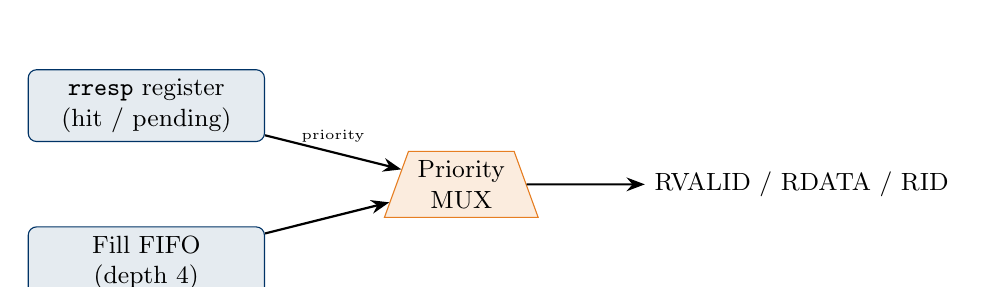
\begin{tikzpicture}[
  box/.style={draw=giki,fill=giki!10,rounded corners=3pt,
              minimum width=3cm,minimum height=0.8cm,
              font=\small,align=center},
  mux/.style={draw=covorange,fill=covorange!15,
              trapezium,trapezium left angle=70,
              trapezium right angle=70,
              minimum width=1.8cm,minimum height=0.6cm,
              font=\small,align=center},
  arr/.style={->,>=Stealth,thick}
]
\node[box] (rresp) at (0,2) {\texttt{rresp} register\\(hit / pending)};
\node[box] (ffq)   at (0,0) {Fill FIFO\\(depth 4)};
\node[mux] (mux)   at (4,1) {Priority\\MUX};
\node[right=1.5cm of mux,font=\small] (out) {RVALID / RDATA / RID};

\draw[arr] (rresp) -- node[above,font=\tiny]{priority} (mux);
\draw[arr] (ffq)   -- (mux);
\draw[arr] (mux)   -- (out);
\end{tikzpicture}
\caption{R-channel response priority multiplexer}
\label{fig:resp_mux}
\end{figure}

% ============================================================
\chapter{Module-Level Design}
\label{ch:design}
% ============================================================

\section{Tag Store}

The tag store is a synchronous SRAM array of dimension
$128 \times 4 \times 22$\,bits.  All four tags for the addressed set
are read combinationally on every cycle and forwarded to the hit
detector.  The read address is driven directly by the arbiter's decoded
\texttt{req\_set} field, so tag data is available in the same cycle as
the request.

Writes occur synchronously on the clock edge following an FSM
allocation (new line installed as PENDING).  The write index always
equals the current request set, and the write way equals the PLRU
victim.  The new tag value is the \texttt{req\_tag} decoded from the
arbiter output.

The tag store does not need a reset: all status bits default to
INVALID (2'b00), so a tag comparison against an INVALID line will
never produce a spurious hit regardless of the stored tag value.
This property is guaranteed by the hit detector's two-condition check
(tag match \emph{and} status VALID).

\section{Status Bits Store}

Each cache line carries a 2-bit status field encoding three states:

\begin{table}[h]
\centering
\caption{Line status encoding}
\label{tab:status}
\begin{tabular}{@{}cll@{}}
\toprule
Encoding & Name & Meaning \\
\midrule
\texttt{2'b00} & INVALID & Line does not hold valid data \\
\texttt{2'b01} & VALID   & Line holds coherent, readable data \\
\texttt{2'b10} & PENDING & Line allocated; memory fetch in progress \\
\bottomrule
\end{tabular}
\end{table}

The status store is a synchronous array of dimension $128 \times 4
\times 2$\,bits, reset to all-INVALID on power-up.  All four statuses
are read combinationally and passed to the hit detector.  The single
write port is shared between two sources:

\begin{enumerate}[label=\arabic*.]
  \item \textbf{FSM}: INVALID$\to$PENDING on miss allocation;
        PENDING$\to$INVALID on write-to-pending cancellation.
  \item \textbf{mm\_rcvd path}: PENDING$\to$VALID on fill completion.
\end{enumerate}

The \texttt{mm\_rcvd} path is evaluated \emph{after} the FSM case
statement in the combinational block, giving it priority over any
FSM-driven status write in the same cycle.  This ordering is
intentional: a fill completion must always advance the status from
PENDING to VALID, even if the FSM simultaneously detects a status
write-port conflict and defers its own write by one cycle.

\section{Hit Detector}

The hit detector is a purely combinational module.  It compares the
incoming tag against all four stored tags and simultaneously checks
the corresponding status bits.  Two independent comparisons are
performed in parallel:

\begin{itemize}
  \item \textbf{True hit}: tag matches \emph{and} status is
        \texttt{2'b01} (VALID).
  \item \textbf{Pending hit}: tag matches \emph{and} status is
        \texttt{2'b10} (PENDING).
\end{itemize}

A priority encoder selects the matching way index for both cases.
The distinction is critical for the non-blocking design:
\begin{itemize}
  \item A pending hit on a \emph{read} means the same line is being
        fetched for a prior miss.  The FSM must stall this second
        read until the fill completes (\textsc{wait\_pending} state),
        after which the fill data is returned directly.
  \item A pending hit on a \emph{write} triggers MSHR cancellation:
        the write supersedes the in-flight fetch, so the MSHR entry
        is cancelled (status $\to$ INVALID) and the write proceeds
        normally via the write buffer.
\end{itemize}

\section{PLRU Store}

\subsection{Tree Structure}

The PLRU store holds one 3-bit tree per set (384 bits total).  Each
bit points \emph{away from} the most recently used subtree as shown
in Figure~\ref{fig:plru}.

\begin{figure}[h]
\centering
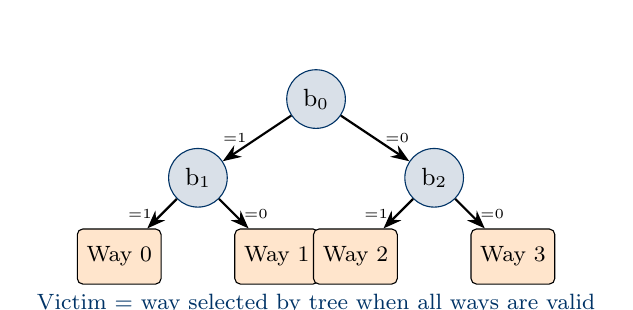
\begin{tikzpicture}[
  nd/.style={circle,draw=giki,fill=giki!15,minimum size=0.7cm,font=\small},
  arr/.style={->,>=Stealth,thick}
]
\node[nd] (root) at (3,2) {b\textsubscript{0}};
\node[nd] (left) at (1.5,1) {b\textsubscript{1}};
\node[nd] (right) at (4.5,1) {b\textsubscript{2}};
\node[draw,rounded corners=2pt,fill=orange!20,minimum size=0.7cm,
      font=\footnotesize] (w0) at (0.5,0) {Way 0};
\node[draw,rounded corners=2pt,fill=orange!20,minimum size=0.7cm,
      font=\footnotesize] (w1) at (2.5,0) {Way 1};
\node[draw,rounded corners=2pt,fill=orange!20,minimum size=0.7cm,
      font=\footnotesize] (w2) at (3.5,0) {Way 2};
\node[draw,rounded corners=2pt,fill=orange!20,minimum size=0.7cm,
      font=\footnotesize] (w3) at (5.5,0) {Way 3};

\draw[arr] (root) -- node[left,font=\tiny]{=1} (left);
\draw[arr] (root) -- node[right,font=\tiny]{=0} (right);
\draw[arr] (left) -- node[left,font=\tiny]{=1} (w0);
\draw[arr] (left) -- node[right,font=\tiny]{=0} (w1);
\draw[arr] (right) -- node[left,font=\tiny]{=1} (w2);
\draw[arr] (right) -- node[right,font=\tiny]{=0} (w3);

\node[font=\footnotesize,color=giki] at (3,-0.6)
  {Victim = way selected by tree when all ways are valid};
\end{tikzpicture}
\caption{3-bit PLRU binary decision tree for a 4-way set}
\label{fig:plru}
\end{figure}

\subsection{Update Rules}

On every cache hit or fill completion, the three bits are updated to
point away from the accessed way:

\begin{table}[h]
\centering
\caption{PLRU bit update rules}
\label{tab:plru_update}
\begin{tabular}{@{}clll@{}}
\toprule
Accessed Way & b\textsubscript{0} & b\textsubscript{1} & b\textsubscript{2} \\
\midrule
Way 0 & 1 & 1 & unchanged \\
Way 1 & 1 & 0 & unchanged \\
Way 2 & 0 & unchanged & 1 \\
Way 3 & 0 & unchanged & 0 \\
\bottomrule
\end{tabular}
\end{table}

The initial tree state \texttt{3'b000} points left-left, selecting
way\,1 as the first victim.  After way\,1 is filled and accessed,
the bits flip to point away from it, selecting way\,3 as the next
victim.  The complete victim sequence from a cold-start with
sequential accesses is: way\,1, way\,3, way\,0, way\,2, then cycling
according to the access history.

\section{Data Store}

The data store is a $128 \times 4 \times 64$-bit synchronous array
(32\,KB) with two independent write ports and one combinational read
port.  The \emph{cpu\_wr} port is asserted on a write hit to update
the cache line in place (write-through).  The \emph{fill\_wr} port is
asserted when \texttt{mm\_rcvd} fires to install the memory response.
These two ports target different ways (VALID for cpu\_wr, PENDING for
fill\_wr) in normal operation, so no arbitration is required.

The read port returns the data for the way selected by
\texttt{hd\_hit\_way} (the true-hit way index).  For read hits the
data is available combinationally in the same cycle as the hit
detection, so it can be registered into the \texttt{rresp} register
on the same edge that \texttt{resp\_en} fires.

\section{Control FSM}
\label{sec:fsm}

\subsection{States and Non-Blocking Property}

The control FSM has three states encoded in two bits, illustrated in
Figure~\ref{fig:fsm_new}.

\begin{figure}[h]
\centering
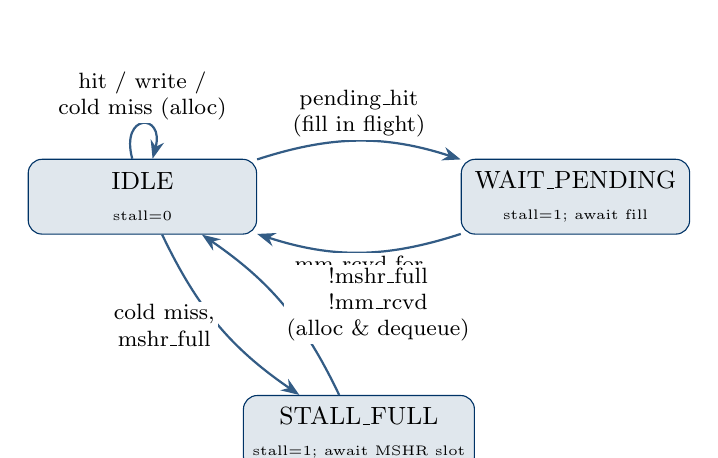
\begin{tikzpicture}[
  st/.style={draw=giki,fill=giki!12,rounded corners=5pt,
             minimum width=2.9cm,minimum height=0.95cm,
             font=\small,align=center},
  tr/.style={->,>=Stealth,thick,color=giki!80},
  lbl/.style={font=\footnotesize,color=black,fill=white,inner sep=1pt,align=center}
]
\node[st] (idle)  at (0,0)    {IDLE\\{\tiny stall=0}};
\node[st] (wait)  at (5.5,0)  {WAIT\_PENDING\\{\tiny stall=1; await fill}};
\node[st] (stall) at (2.75,-3) {STALL\_FULL\\{\tiny stall=1; await MSHR slot}};

% Self-loop on IDLE
\draw[tr] (idle) to[loop above,looseness=6]
    node[lbl,above]{hit / write /\\cold miss (alloc)} (idle);

% IDLE -> WAIT_PENDING
\draw[tr] (idle) to[bend left=18]
    node[lbl,above]{pending\_hit\\(fill in flight)} (wait);

% WAIT_PENDING -> IDLE
\draw[tr] (wait) to[bend left=18]
    node[lbl,below]{mm\_rcvd for\\req\_set} (idle);

% IDLE -> STALL_FULL
\draw[tr] (idle) to[bend right=15]
    node[lbl,left]{cold miss,\\mshr\_full} (stall);

% STALL_FULL -> IDLE (non-blocking)
\draw[tr] (stall) to[bend right=15]
    node[lbl,right]{!mshr\_full\\!mm\_rcvd\\(alloc \& dequeue)} (idle);

\end{tikzpicture}
\caption{3-state non-blocking control FSM — state transition diagram}
\label{fig:fsm_new}
\end{figure}

The key property is that \textbf{cold misses do not leave the IDLE
state}.  The FSM allocates an MSHR entry, writes the tag and PENDING
status, and remains in IDLE---all in the same cycle that
\texttt{mshr\_alloc\_en} fires and dequeues the request.  The fill
will complete asynchronously; the pipeline proceeds with the next
request.

\subsection{IDLE State Behaviour}

The IDLE state handles all transaction types combinationally each
cycle.  Priority ordering within the read path is:

\begin{enumerate}[label=\arabic*.]
  \item \textbf{Write buffer hit} (\texttt{wb\_hit}): return forwarded
        data immediately via \texttt{resp\_en=1, fwd\_sel=1}; no cache
        array access.
  \item \textbf{True hit} (\texttt{true\_hit}): assert \texttt{resp\_en},
        update PLRU.
  \item \textbf{Pending hit} (\texttt{pending\_hit}):
        \begin{itemize}
          \item If \texttt{mm\_rcvd} is simultaneously asserted for
                the same set, resolve immediately with
                \texttt{pending\_resolved=1} (no stall).
          \item Otherwise, stall (\texttt{stall=1}) and transition
                to \textsc{wait\_pending}.
        \end{itemize}
  \item \textbf{Cold miss}:
        \begin{itemize}
          \item If \texttt{mshr\_full}, stall and go to
                \textsc{stall\_full}.
          \item If \texttt{mm\_rcvd} is asserted (status write-port
                busy), stall for exactly one cycle.
          \item Otherwise, assert \texttt{mshr\_alloc\_en}, write tag
                and PENDING status, remain in IDLE.  The arbiter
                dequeues the request this same cycle.
        \end{itemize}
\end{enumerate}

For writes (write-through, no-write-allocate):
\begin{enumerate}[label=\arabic*.]
  \item Push to write buffer (\texttt{wb\_push\_en=1}) if not full.
        Write buffer full $\to$ stall.
  \item If true hit: additionally update data store (\texttt{cpu\_data\_wr\_en})
        and PLRU.
  \item If pending hit: cancel the in-flight MSHR entry
        (\texttt{mshr\_dealloc\_en}, status $\to$ INVALID) to prevent
        stale fill data from overwriting the new write value.
\end{enumerate}

\subsection{WAIT\_PENDING State}

The FSM enters \textsc{wait\_pending} when a read targets a line
whose fill is already in flight (pending hit detected in IDLE, no
simultaneous \texttt{mm\_rcvd} resolution).  In this state
\texttt{stall=1} is asserted, preventing the arbiter from loading a
new request.

When \texttt{mm\_rcvd} fires for the stalled set (\texttt{mm\_rcvd\_set
== req\_set}), the FSM:
\begin{itemize}
  \item Returns to IDLE.
  \item Asserts \texttt{pending\_resolved=1} for one cycle.
  \item Deasserts \texttt{stall}.
\end{itemize}

\texttt{cache\_top} captures \texttt{fill\_data} and \texttt{req\_id}
into the \texttt{rresp} register on the \texttt{pending\_resolved}
pulse, generating the correct R response for the stalled request.
\texttt{out\_ready} fires via \texttt{pending\_resolved}, dequeuing
the request.

Note that the FSM also processes the fill via the \texttt{mm\_rcvd}
block (status store update, data store write).  The pending-resolved
response path and the fill-notification path are therefore concurrent
in the same cycle.

\subsection{STALL\_FULL State}

The FSM enters \textsc{stall\_full} when all four MSHR entries are
occupied and a new cold miss arrives.  With the non-blocking design,
this state is \emph{reachable}: up to four misses can be independently
in flight simultaneously (one per MSHR entry), so a fifth miss
genuinely encounters a full MSHR.

The FSM waits in \textsc{stall\_full} until an MSHR slot becomes free
(\texttt{!mshr\_full}) and the status write port is available
(\texttt{!mm\_rcvd}).  It then allocates the MSHR, writes the tag and
PENDING status, and returns directly to IDLE---exactly the same
non-blocking path as a normal cold miss.

\subsection{mm\_rcvd Block}

The final section of the \texttt{always\_comb} block is an
unconditional \texttt{if (mm\_rcvd)} clause that executes
\emph{regardless of the current FSM state}.  This clause:

\begin{lstlisting}[style=sv]
if (mm_rcvd) begin
    status_wr_en   = 1'b1;
    status_wr_set  = mm_rcvd_set;
    status_wr_way  = mm_rcvd_way;
    status_wr_data = VALID;        // PENDING -> VALID
    fill_data_wr_en = 1'b1;
end
\end{lstlisting}

\noindent overrides any FSM-driven status write in the same cycle
because it appears after the \texttt{case} statement.  This ensures
fill completion always wins the status write-port arbitration.

\section{Round-Robin Arbiter}
\label{sec:arbiter}

\subsection{Design}

Two independent FIFOs of depth~8 buffer AR and AW+W requests before
the arbiter.  The arbiter maintains a single \texttt{last\_served} bit
and grants access to the opposite channel on each new arbitration,
providing strict round-robin fairness.  It is a hold-until-acknowledge
design: its output remains valid until \texttt{out\_ready} asserts.

\subsection{FIFO Re-Presentation Guard}

A subtle correctness requirement arises from the non-blocking design.
When \texttt{out\_ready} and a new FIFO entry coincide in the same
cycle, the arbiter must \emph{not} re-load the FIFO entry that was
just popped.  Without a guard, the following race can occur:

\begin{enumerate}[label=\arabic*.]
  \item Cycle $N$: \texttt{mshr\_alloc\_en=1} $\Rightarrow$
        \texttt{out\_ready=1}.  Arbiter drives \texttt{r\_ready=1},
        popping the read FIFO.
  \item At the NBA phase of cycle $N$, the FIFO's count decrements.
        But at the active edge of cycle $N$, the arbiter samples
        \texttt{r\_valid} using the \emph{pre-decrement} (stale) count.
  \item The arbiter sees stale \texttt{r\_valid=1} and re-loads the
        same FIFO entry on the next cycle --- duplicating the request.
\end{enumerate}

The fix is to guard the FIFO reload condition with the pop strobe:

\begin{lstlisting}[style=sv]
out_valid <= r_valid && !r_ready;   // was: r_valid
r_ready   <= r_valid && !r_ready;
\end{lstlisting}

When \texttt{r\_ready} is already asserted (the pop is in progress),
\texttt{out\_valid} is forced low, preventing re-presentation.  The
same guard applies to the write FIFO (\texttt{w\_ready}).

\section{MSHR}
\label{sec:mshr}

\subsection{Entry Lifecycle}

Figure~\ref{fig:mshr_fsm} shows the three-state lifecycle of each
MSHR entry.

\begin{figure}[h]
\centering
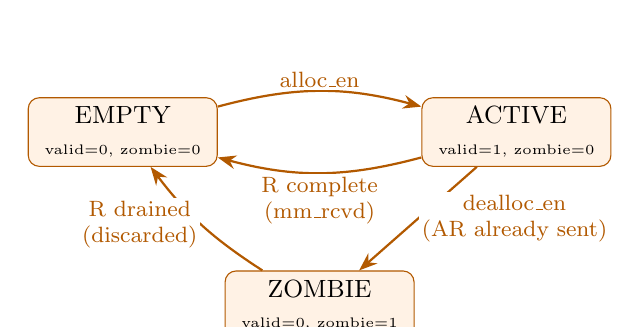
\begin{tikzpicture}[
  st/.style={draw=orange!70!black,fill=orange!10,rounded corners=4pt,
             minimum width=2.4cm,minimum height=0.8cm,
             font=\small,align=center},
  tr/.style={->,>=Stealth,thick,color=orange!70!black},
  lbl/.style={font=\footnotesize,fill=white,inner sep=1pt,align=center}
]
\node[st] (empty)  at (0,0)    {EMPTY\\{\tiny valid=0, zombie=0}};
\node[st] (active) at (5,0)    {ACTIVE\\{\tiny valid=1, zombie=0}};
\node[st] (zombie) at (2.5,-2.2) {ZOMBIE\\{\tiny valid=0, zombie=1}};

\draw[tr] (empty)  to[bend left=15]
    node[lbl,above]{alloc\_en} (active);
\draw[tr] (active) to[bend left=15]
    node[lbl,below]{R complete\\(mm\_rcvd)} (empty);
\draw[tr] (active) -- node[lbl,right]{dealloc\_en\\(AR already sent)} (zombie);
\draw[tr] (zombie) to[bend left=10]
    node[lbl,left]{R drained\\(discarded)} (empty);
\end{tikzpicture}
\caption{MSHR entry state transitions}
\label{fig:mshr_fsm}
\end{figure}

\subsection{AXI Read Master}

The MSHR acts as an AXI4 read master toward main memory.  The entry
index (0--3) is used as the AXI transaction ID (\texttt{ARID}), so
the R-channel response can be matched back to the correct entry using
\texttt{RID[1:0]}.  At most one AR request is issued at a time (the
lowest-indexed pending entry without \texttt{ar\_sent=1}).
\texttt{RREADY} is permanently asserted.

With up to four MSHR entries active simultaneously, the MSHR issues
AR requests in lowest-index-first order.  Each entry's AR is sent
independently; the main memory model responds to each in order.  The
\texttt{ar\_sent} flag prevents an entry from being re-issued once
its AR has been accepted.

\subsection{Zombie State}

The \emph{zombie} state handles a timing edge case for the write-to-pending
cancellation: if the FSM cancels an entry via \texttt{dealloc\_en}
\emph{after} its AR has already been accepted by main memory
(\texttt{ar\_sent=1}), the R response is already in flight.  The
MSHR cannot silently discard it because the AXI bus would stall.
The zombie state allows the MSHR to receive and discard the R response
cleanly without asserting \texttt{mm\_rcvd}.

\subsection{Multi-Entry Operation}

With the non-blocking FSM, up to four read misses can be outstanding
simultaneously.  The MSHR allocates a new entry for each, issues
their ARs in order, and fires \texttt{mm\_rcvd} for each R response.
The fill FIFO in \texttt{cache\_top} absorbs up to four simultaneous
\texttt{mm\_rcvd} pulses (depth 4 matches MSHR capacity), ensuring no
fill response is dropped even if the CPU R channel is occupied.

\section{Write Buffer}
\label{sec:wbuf}

\subsection{Structure}

The write buffer is an 8-entry FIFO.  Each entry stores address, data,
write strobe, and transaction ID.  A combinational scan from newest
to oldest entry provides RAW forwarding: if the read address matches
any live entry, the newest matching data is returned.

\subsection{AXI Write Master FSM}

\begin{figure}[h]
\centering
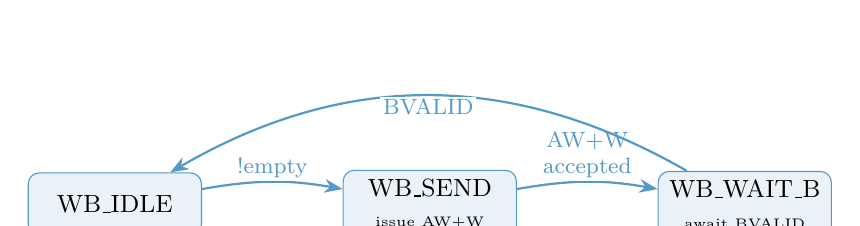
\begin{tikzpicture}[
  st/.style={draw=covblue!80,fill=covblue!10,rounded corners=4pt,
             minimum width=2.2cm,minimum height=0.8cm,
             font=\small,align=center},
  tr/.style={->,>=Stealth,thick,color=covblue!80},
  lbl/.style={font=\footnotesize,fill=white,inner sep=1pt,align=center}
]
\node[st] (idle) at (0,0)  {WB\_IDLE};
\node[st] (send) at (4,0)  {WB\_SEND\\{\tiny issue AW+W}};
\node[st] (wait) at (8,0)  {WB\_WAIT\_B\\{\tiny await BVALID}};

\draw[tr] (idle) to[bend left=10]
    node[lbl,above]{!empty} (send);
\draw[tr] (send) to[bend left=10]
    node[lbl,above]{AW+W\\accepted} (wait);
\draw[tr] (wait) to[bend right=30]
    node[lbl,below]{BVALID} (idle);
\end{tikzpicture}
\caption{Write buffer drain state machine}
\label{fig:wbuf_fsm}
\end{figure}

\noindent\textbf{Important:} The CPU B response (\texttt{BVALID}
toward the master) is forwarded directly from the main-memory B
channel.  The CPU therefore observes the full main-memory write
latency.  This differs from designs that assert \texttt{BVALID}
immediately on write-buffer acceptance; the current approach is
simpler but less effective at hiding write latency from the
perspective of the processor awaiting the B response.

\subsection{RAW Forwarding}

The RAW forwarding comparator scans all live write buffer entries on
every cycle.  Because writes are accepted immediately into the buffer
(via \texttt{wb\_push\_en}), a read issued on the very next cycle will
see the write's data in the buffer and return it directly.  This
guarantees read-after-write coherence without requiring the processor
to wait for the write to reach main memory.

\section{Fill Response FIFO}
\label{sec:fill_fifo}

The fill response FIFO is a depth-4 synchronous FIFO implemented
directly in \texttt{cache\_top}.  Each entry is $64 + 4 = 68$ bits
wide, storing the 64-bit fill data concatenated with the 4-bit CPU
AXI ID of the original miss request.

\textbf{Push:} \texttt{fq\_push = mm\_rcvd}.  Every fill
notification immediately enqueues the fill data and CPU ID.

\textbf{Pop:} \texttt{fq\_pop = fq\_valid \&\& !rresp\_valid \&\&
s\_axi\_rready}.  The FIFO drains to the R channel only when the
\texttt{rresp} register is empty and the CPU is ready to accept a
response.

\textbf{Depth:} Four entries match the MSHR capacity.  In the worst
case, four fills complete back-to-back while the CPU R channel is
occupied by a \texttt{rresp} hit response.  The FIFO absorbs all four
fill completions without overflow.

The FIFO implements simple power-of-two pointer arithmetic.  The read
pointer and write pointer are each 2 bits wide; a 3-bit count register
tracks occupancy and drives \texttt{fq\_valid}.

\section{Main Memory Model}

The main memory is a behavioural SystemVerilog model with 65\,536
entries of 64 bits each (512\,KB addressable range).  It responds to
both read and write AXI channels with a single-cycle latency and
permanently asserted \texttt{ARREADY}, \texttt{AWREADY}, and
\texttt{WREADY} signals, simulating an ideal memory.  The testbench
pre-loads entries via hierarchical reference (\texttt{dut.u\_mm.mem})
to seed known values before each test group.

\section{Known Limitations}
\label{sec:limitations}

\begin{enumerate}[label=\arabic*.]
  \item \textbf{AW+W simultaneous requirement.}  The current
        implementation requires AW and W to be driven in the same
        clock cycle.  An \texttt{axi\_merger} module capable of
        handling skewed arrivals was developed but not integrated due
        to a bug in its address capture logic.  Fixing this is
        identified as future work.
  \item \textbf{Single-beat cache lines.}  Each cache line is exactly
        one 64-bit AXI beat.  Wider cache lines would improve spatial
        locality but require a burst-capable MSHR and multi-beat data
        store.
  \item \textbf{No write-back support.}  Adding a dirty bit and
        eviction path would reduce write bandwidth to main memory at
        the cost of additional hardware and a more complex eviction
        FSM.
  \item \textbf{No out-of-order R responses.}  The fill FIFO delivers
        responses in fill-completion order, not in the order of the
        original AR requests.  A compliant AXI4 master must tolerate
        out-of-order R responses (using the RID field to match
        responses to requests), which the testbench does.
\end{enumerate}

% ============================================================
\chapter{Verification}
\label{ch:verification}
% ============================================================

\section{Testbench Architecture}

The testbench instantiates \texttt{cache\_top} as the device under
test (DUT) and drives it through its CPU-facing AXI4 slave interface.
The main memory model is instantiated \emph{inside} the DUT, and the
testbench pre-seeds it via hierarchical reference before each test
group.

Two reusable tasks implement the AXI handshake protocol:
\texttt{axi\_read} and \texttt{axi\_write}.  Both include a per-cycle
timeout counter that fails the test gracefully if an expected handshake
does not occur within 200 cycles.  All expected data values are checked
via a \texttt{check} task that increments either the pass or fail
counter.  A third task, \texttt{axi\_read\_nb} (non-blocking), issues
an AR without waiting for RVALID, enabling concurrent request issuance
in TC8 and TC9.

\section{Test Cases}
\label{sec:tcs}

Table~\ref{tab:tcs} summarises all ten test cases.

\begin{table}[h]
\centering
\caption{Directed test case summary}
\label{tab:tcs}
\begin{tabularx}{\linewidth}{@{}llX@{}}
\toprule
Test Case & Assertions & Scenario \\
\midrule
TC1  & 2 & Cold read miss; second read is a true hit \\
TC2  & 3 & Write primes MM; read fills from MM; second read is a hit \\
TC3  & 6 & Four consecutive reads to the same set (4 different tags),
           filling all PLRU victim paths; two re-reads verify hits \\
TC4  & 4 & Four consecutive writes; B response received for each \\
TC5  & 4 & Mixed: read miss, write miss, read hit, write miss \\
TC6  & 1 & RAW forwarding: write without waiting for B, immediate
           read returns write-buffer value rather than MM value \\
TC7  & 2 & Write hit: write to an already-valid cache line, read back
           confirms data store updated \\
TC8  & 2 & Hit-under-miss: read miss to set A; before fill completes,
           read hit to set B (already valid); both responses correct \\
TC9  & 2 & Concurrent misses: two reads to different sets, both miss;
           two independent MSHR entries allocated; both fills complete \\
TC10 & 1 & Pending-hit stall: read miss to set C; second read to same
           address; FSM enters WAIT\_PENDING; fill data returned for both \\
\midrule
\textbf{Total} & \textbf{27} & \\
\bottomrule
\end{tabularx}
\end{table}

\section{Test Case Descriptions}

\subsection{TC1 — Read Miss Followed by Hit}

The testbench pre-loads main memory at address \texttt{(tag=0, set=0)}
with the value \texttt{0xCAFE0001DEAD0001}.  The first
\texttt{axi\_read} generates a cold miss: the MSHR allocates entry~0,
the arbiter dequeues the request immediately (\texttt{mshr\_alloc\_en}
fires), and an AXI AR is issued to main memory.  When the R response
arrives, \texttt{mm\_rcvd} fires, the fill FIFO is pushed, and the
status transitions to VALID.  The CPU receives RVALID from the fill
FIFO.  The second \texttt{axi\_read} to the same address hits in the
now-VALID line and is served in a single cycle from the data store.

\subsection{TC2 — Write Then Read}

This test establishes that a write followed by a read correctly
populates the cache via a fill.  An \texttt{axi\_write} to address
\texttt{(tag=0, set=1)} pushes to the write buffer and propagates to
main memory.  A subsequent \texttt{axi\_read} to the same address
misses (the write did not allocate the cache line) and triggers a fill
from main memory.  The fill returns the most recently written value.
A second read is a true hit.  Three assertions verify: fill response
data, hit response data, and B response received for the write.

\subsection{TC3 — PLRU Victim Coverage}

TC3 exercises all four PLRU victim paths in a single set.  Four
sequential reads to set~2 with distinct tags fill all four ways in
PLRU victim order (way\,1, way\,3, way\,0, way\,2 from initial state
\texttt{3'b000}).  Two additional reads to the first and third
addresses verify that the corresponding lines remain valid (no
spurious eviction).  Six assertions check: four fill responses and two
re-hit responses.

\subsection{TC4 — Consecutive Writes}

TC4 verifies write-buffer throughput.  Four consecutive writes to
distinct addresses are accepted into the write buffer without stalling
(the write buffer has 8 slots and is empty at the start of TC4).
Each write is followed by waiting for the B response from main memory,
confirming end-to-end write drain.  Four assertions check that each B
response is received.

\subsection{TC5 — Mixed Read/Write}

TC5 interleaves reads and writes.  A read miss to a fresh address is
followed by a write miss, a read hit (the line from the first read is
now valid), and a second write miss.  This test exercises the
write-through path alongside read-miss allocation and hit servicing
within a single sequence.  Four assertions verify the read miss fill
data, two B responses, and the read hit data.

\subsection{TC6 — RAW Forwarding}

TC6 verifies the write-buffer forwarding path.  A write is issued to
address \texttt{(tag=0, set=5)} \emph{without} waiting for the B
response (so the write buffer entry is still live).  An immediately
following read to the same address must return the write-buffer data
(\texttt{0xFEEDFACEFEEDFACE}) rather than the MM seed value
(\texttt{0xDEADDEADDEADDEAD}).  The FSM detects \texttt{wb\_hit=1}
and asserts \texttt{fwd\_sel=1}, bypassing the data store and main
memory entirely.  One assertion checks the returned data value.

\subsection{TC7 — Write Hit}

TC7 exploits the fact that the line at \texttt{(tag=0, set=0)} loaded
in TC1 remains valid throughout all subsequent tests.  A write to the
same address triggers the write-hit path: \texttt{cpu\_data\_wr\_en}
updates the data store in place and \texttt{wb\_push\_en} forwards the
write to the write buffer (write-through).  A subsequent read confirms
the data store holds the new value \texttt{0xCAFEBABE12345678}.

\subsection{TC8 — Hit Under Miss}
\label{sec:tc8}

TC8 is the canonical non-blocking test.  It pre-loads main memory
at two addresses: \texttt{(tag=5, set=10)} and \texttt{(tag=0, set=0)}
(the latter already valid from TC1 and TC7).

\begin{enumerate}[label=\arabic*.]
  \item An AR is issued to \texttt{(tag=5, set=10)}: cold miss.
        MSHR allocates entry~0; \texttt{mshr\_alloc\_en=1}; the
        arbiter dequeues the request; \texttt{stall=0}.
  \item Before the fill completes, an AR is issued to
        \texttt{(tag=0, set=0)}: true hit (valid from prior tests).
        The FSM serves the hit normally in IDLE, asserting
        \texttt{resp\_en}.  The hit response is registered into
        \texttt{rresp}.
  \item The fill for set~10 arrives; \texttt{mm\_rcvd} fires;
        fill FIFO receives the data.  The fill FIFO delivers the
        response on the R channel after the hit response.
\end{enumerate}

Two assertions verify that both reads return the correct data.
The absence of any stall between the two ARs (observable in the
waveform) is the key correctness property.

\subsection{TC9 — Concurrent Misses}
\label{sec:tc9}

TC9 verifies that the MSHR correctly manages two independent
outstanding misses.  Two reads are issued back-to-back to
\texttt{(tag=7, set=12)} and \texttt{(tag=8, set=13)}, both cold
misses.

\begin{enumerate}[label=\arabic*.]
  \item AR1 arrives at the FSM: cold miss.  MSHR allocates entry~0;
        \texttt{mshr\_alloc\_en=1}; request dequeued; \texttt{stall=0}.
  \item AR2 arrives at the FSM (next cycle): cold miss.  MSHR
        allocates entry~1; request dequeued; \texttt{stall=0}.
  \item The MSHR issues ARs to main memory for entries 0 and 1.
        Two \texttt{mm\_rcvd} pulses fire on successive cycles.
        Both push into the fill FIFO.
  \item The fill FIFO delivers two RVALID responses.
\end{enumerate}

Two assertions check that each read receives its own fill data.
The test confirms that the fill FIFO correctly tracks two entries
and that the CPU AXI IDs are correctly associated with each fill.

\subsection{TC10 — Pending-Hit Stall}
\label{sec:tc10}

TC10 exercises the \textsc{wait\_pending} FSM state.  The test
pre-loads main memory at \texttt{(tag=9, set=20)}.

\begin{enumerate}[label=\arabic*.]
  \item AR1 to \texttt{(tag=9, set=20)}: cold miss.  MSHR allocates;
        request dequeued; line status = PENDING; \texttt{stall=0}.
  \item AR2 to the \emph{same} address: hit detector sees PENDING
        status (\texttt{pending\_hit=1}).  FSM checks if
        \texttt{mm\_rcvd} is simultaneously asserted for set~20; it
        is not, since the fill is still in flight.  FSM asserts
        \texttt{stall=1} and transitions to \textsc{wait\_pending}.
  \item \texttt{mm\_rcvd} fires for set~20.  FSM returns to IDLE,
        asserts \texttt{pending\_resolved=1}.  \texttt{cache\_top}
        latches fill data into \texttt{rresp}.
  \item The fill FIFO also received the \texttt{mm\_rcvd} push (for
        AR1).  The \texttt{rresp} register (AR2) has priority on the
        R channel.  AR2 receives the fill data first; AR1's response
        follows from the fill FIFO.
\end{enumerate}

One assertion checks that AR2 receives the correct fill data via the
pending-resolved path.

\section{Functional Coverage}
\label{sec:coverage}

\subsection{Coverage Groups}

Seven SystemVerilog covergroups were written in the testbench and
sampled at \texttt{posedge clk}.  Hierarchical references access
internal signals through the DUT hierarchy.

\begin{table}[htbp]
\centering\small
\caption{Covergroup definitions}
\label{tab:covgroups}
\begin{tabularx}{\linewidth}{@{}>{\ttfamily\small}l>{\raggedright\arraybackslash}X>{\raggedright\arraybackslash}X@{}}
\toprule
\normalfont Covergroup & Coverpoints & What is verified \\
\midrule
read\_scenarios\_cg    & 5 (true hit, WB fwd, miss alloc, pending hit,
                          MSHR-full stall)                            & All read pipeline outcomes \\
write\_scenarios\_cg   & 4 (write hit, write miss, write-to-pending,
                          WB-full stall)                              & All write pipeline outcomes \\
plru\_victim\_cg       & 4 (way 0--3)                                & All four PLRU victim ways selected \\
fill\_cg               & 1 (\normalfont\texttt{mm\_rcvd} pulse)      & Memory fill completion observed \\
rw\_hit\_cross\_cg     & \normalfont Cross: \{read,write\} $\times$ \{hit,miss\} & All four R/W$\times$hit/miss combinations \\
nonblocking\_cg        & 2 (\normalfont\texttt{mshr\_alloc\_en} while
                          \normalfont\texttt{stall=0}; fill FIFO pop) & Non-blocking miss dequeue and fill delivery \\
fill\_fifo\_depth\_cg  & 3 (single fill, double fill, FIFO pop)      & Fill FIFO occupancy scenarios \\
\bottomrule
\end{tabularx}
\end{table}

\subsection{Non-Blocking Covergroup}

The \texttt{nonblocking\_cg} covergroup specifically verifies the
non-blocking property.  Its two coverpoints are:

\begin{lstlisting}[style=sv]
covergroup nonblocking_cg @(posedge clk);
  // Cold miss dequeued without stall
  nb_miss: coverpoint (dut.u_fsm.mshr_alloc_en &&
                       !dut.u_fsm.stall) {
      bins alloc_no_stall = {1};
  }
  // Fill FIFO delivers a fill response
  fill_fifo_pop: coverpoint dut.fq_pop {
      bins pop = {1};
  }
endgroup
\end{lstlisting}

Both bins are hit by TC1 (the first cold miss) and every subsequent
miss TC, confirming the non-blocking path is exercised.

\subsection{Tool Setup}

Simulation was run on Cadence Xcelium 25.03 via EDA Playground with
the following options:

\begin{lstlisting}[style=sv,language=,numbers=none]
xrun -coverage all -covoverwrite -access +rwc
     design.sv testbench.sv
\end{lstlisting}

The \texttt{-coverage all} flag enables statement, branch, toggle, and
functional (covergroup) instrumentation.  The \texttt{-access +rwc}
flag grants read/write/connect access to all hierarchy, required for
covergroup hierarchical references.

% ============================================================
\chapter{Results and Discussion}
\label{ch:results}
% ============================================================

\section{Simulation Results}

All 27 assertions across ten test cases passed with zero failures.
Simulation completed at 2\,260\,ns of simulated time.

\begin{table}[h]
\centering
\caption{Simulation pass/fail summary}
\label{tab:sim_results}
\begin{tabular}{@{}lrr@{}}
\toprule
Test Case & Assertions & Outcome \\
\midrule
TC1  — Read miss + hit           & 2  & \textcolor{covgreen}{\textbf{PASS}} \\
TC2  — Write then read           & 3  & \textcolor{covgreen}{\textbf{PASS}} \\
TC3  — 4 reads same set          & 6  & \textcolor{covgreen}{\textbf{PASS}} \\
TC4  — 4 consecutive writes      & 4  & \textcolor{covgreen}{\textbf{PASS}} \\
TC5  — Mixed read/write          & 4  & \textcolor{covgreen}{\textbf{PASS}} \\
TC6  — RAW forwarding            & 1  & \textcolor{covgreen}{\textbf{PASS}} \\
TC7  — Write hit                 & 2  & \textcolor{covgreen}{\textbf{PASS}} \\
TC8  — Hit under miss            & 2  & \textcolor{covgreen}{\textbf{PASS}} \\
TC9  — Concurrent misses         & 2  & \textcolor{covgreen}{\textbf{PASS}} \\
TC10 — Pending-hit stall         & 1  & \textcolor{covgreen}{\textbf{PASS}} \\
\midrule
\textbf{Total}                   & \textbf{27} & \textbf{27 PASS / 0 FAIL} \\
\bottomrule
\end{tabular}
\end{table}

\section{Simulation Waveforms}

The following waveforms illustrate the five most significant
transaction scenarios in the non-blocking design.  Signals follow the
internal \texttt{cache\_top} wire naming conventions.

\subsection{TC1 — Non-Blocking Read Miss}

Figure~\ref{fig:wv_miss} shows the full sequence of a cold read miss
with non-blocking dequeue.  When \texttt{arvalid} is asserted, the
FSM detects no matching valid line and allocates an MSHR entry:
\texttt{mshr\_alloc\_en} fires for one cycle.  Because
\texttt{mshr\_alloc\_en} is part of \texttt{out\_ready}, the arbiter
simultaneously pops the read FIFO.  \texttt{stall} remains deasserted
throughout.  The MSHR issues \texttt{mshr\_arvalid} to main memory.
When the R response arrives, \texttt{mm\_rcvd} pulses for one cycle,
\texttt{fq\_push} pushes the fill data into the fill FIFO, and
\texttt{fq\_valid} asserts.  \texttt{RVALID} fires on the R channel
as the fill FIFO drains.  The entire cold-miss sequence from arbiter
dequeue to RVALID takes approximately 4--5 clock cycles.  Crucially,
\texttt{stall} is never asserted, so the pipeline is free to accept
new requests during the fill.

\begin{figure}[htbp]
\centering
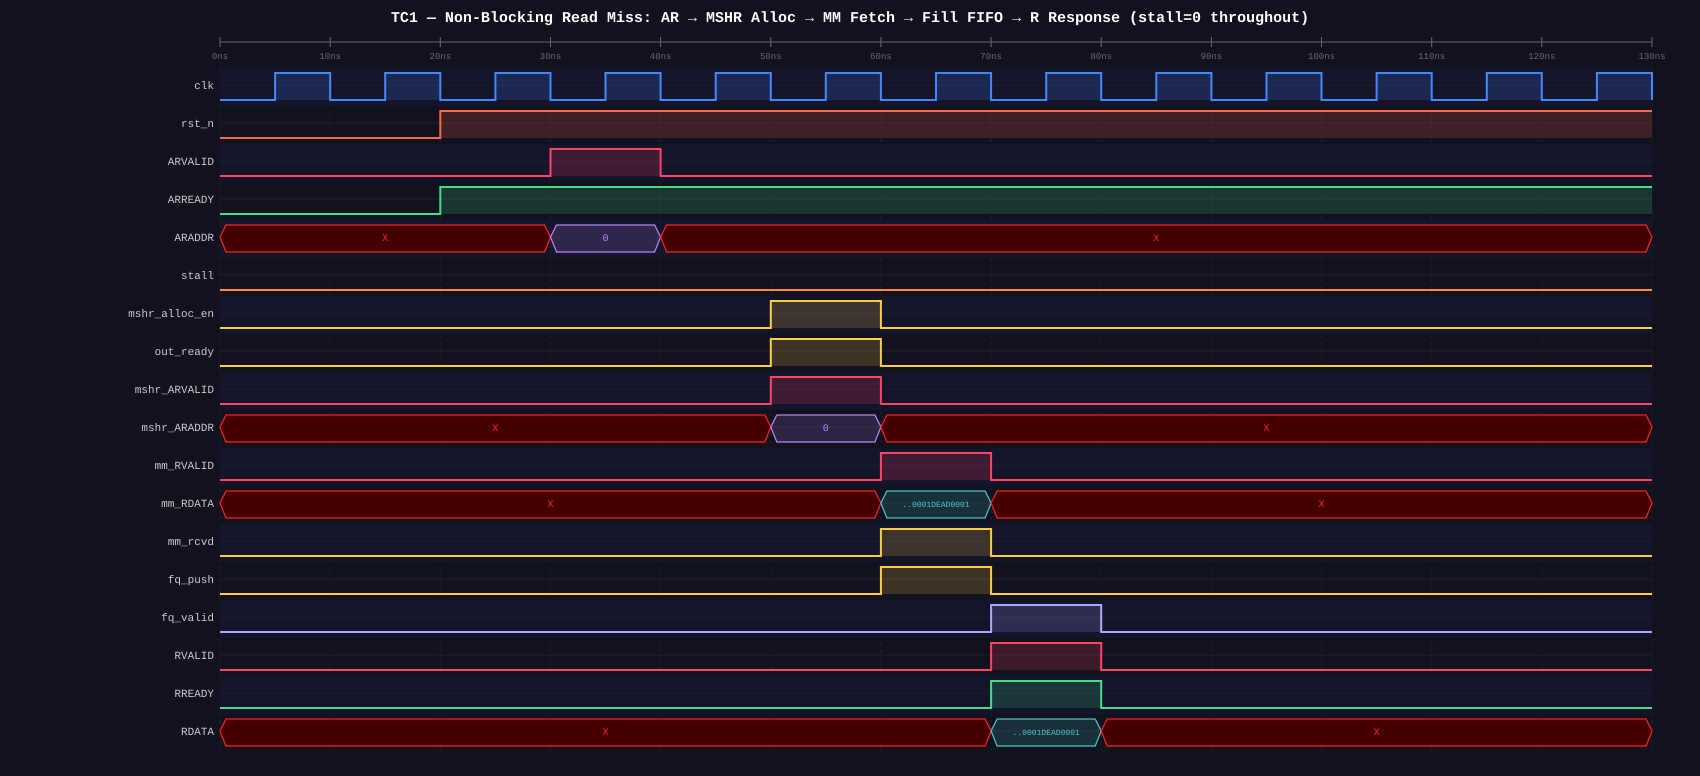
\includegraphics[width=\linewidth]{waveforms/01_tc1_read_miss.pdf}
\caption{TC1: Non-blocking cold read miss --- \texttt{mshr\_alloc\_en} dequeues
         the request at miss time; \texttt{stall=0} throughout; fill data
         delivered via fill FIFO on \texttt{mm\_rcvd}}
\label{fig:wv_miss}
\end{figure}

\subsection{TC1 — Subsequent Cache Hit}

Figure~\ref{fig:wv_hit} shows the second read to the same address
immediately after the fill.  The tag store now holds a matching tag
with status VALID, so \texttt{hd\_hit} asserts combinationally.  The
FSM asserts \texttt{resp\_en}; the data store output is registered
into \texttt{rresp\_valid} on the next clock edge.  \texttt{RVALID}
fires one cycle after ARVALID, confirming single-cycle hit latency
with no memory access.

\begin{figure}[htbp]
\centering
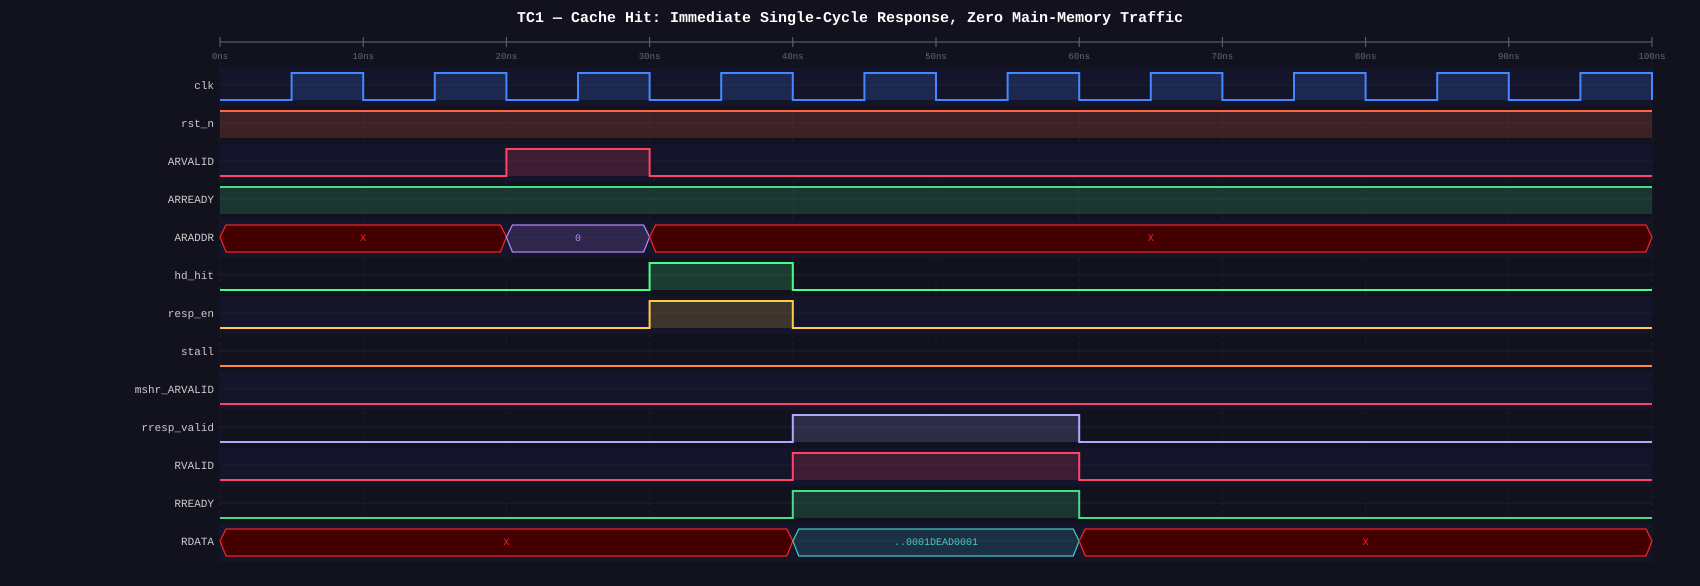
\includegraphics[width=\linewidth]{waveforms/02_tc1_cache_hit.pdf}
\caption{TC1: Cache hit --- \texttt{hd\_hit} asserts immediately;
         \texttt{resp\_en} fires; data returned via \texttt{rresp} register
         with single-cycle latency}
\label{fig:wv_hit}
\end{figure}

\subsection{TC8 — Hit Under Miss}

Figure~\ref{fig:wv_hum} demonstrates hit-under-miss operation: the
defining property of a non-blocking cache.  AR1 to an unmapped address
generates a cold miss (\texttt{mshr\_alloc\_en} fires; stall=0).
Before the fill completes, AR2 to a previously valid address is
processed in the next cycle.  The hit detector asserts \texttt{hd\_hit}
for AR2; \texttt{resp\_en} fires; the hit data is registered into
\texttt{rresp\_valid}.  The cache serves a hit response \emph{while
the fill for AR1 is still outstanding}.  When the fill completes,
\texttt{fq\_push} pushes it into the fill FIFO; the two responses
appear on the R channel in order (hit first, then fill).

\begin{figure}[htbp]
\centering
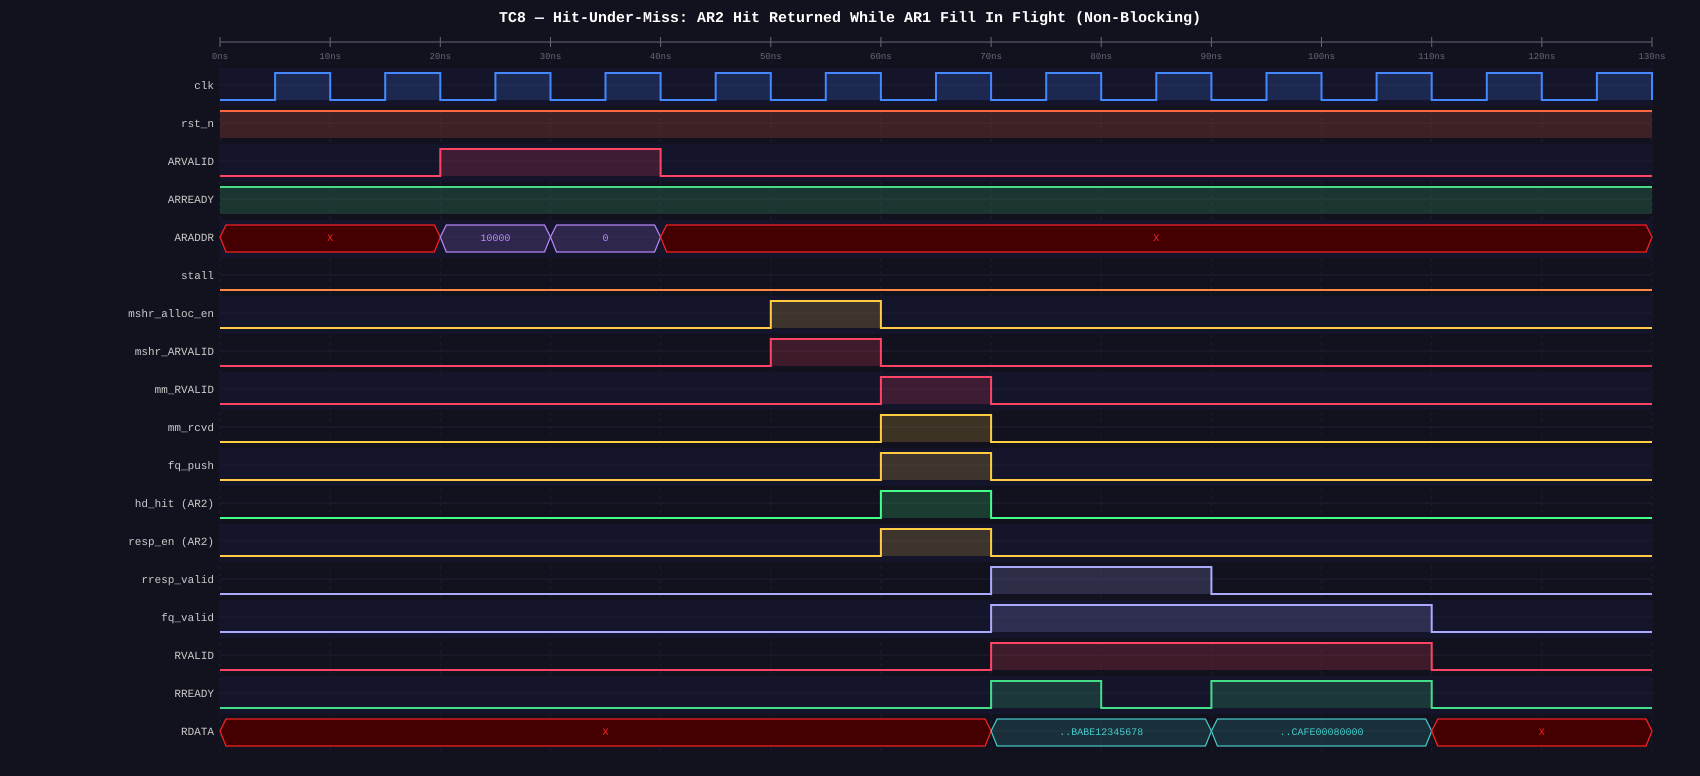
\includegraphics[width=\linewidth]{waveforms/03_tc8_hit_under_miss.pdf}
\caption{TC8: Hit under miss --- AR2 (hit) is served while AR1 fill is
         in flight; \texttt{stall=0} throughout; both responses correct}
\label{fig:wv_hum}
\end{figure}

\subsection{TC9 — Concurrent Misses}

Figure~\ref{fig:wv_conc} shows two independent cold misses to
different sets processed back-to-back.  Both ARs result in
\texttt{mshr\_alloc\_en} pulses on consecutive cycles (MSHR entries~0
and~1 allocated).  The MSHR issues ARs to main memory in
lowest-index-first order.  Both fills complete and generate
\texttt{mm\_rcvd} pulses; both push to the fill FIFO.  The fill FIFO
count reaches 2, then drains as RVALID fires twice on the R channel.
\texttt{stall} remains deasserted throughout both miss allocations,
confirming that the non-blocking property extends to multiple
outstanding misses.

\begin{figure}[htbp]
\centering
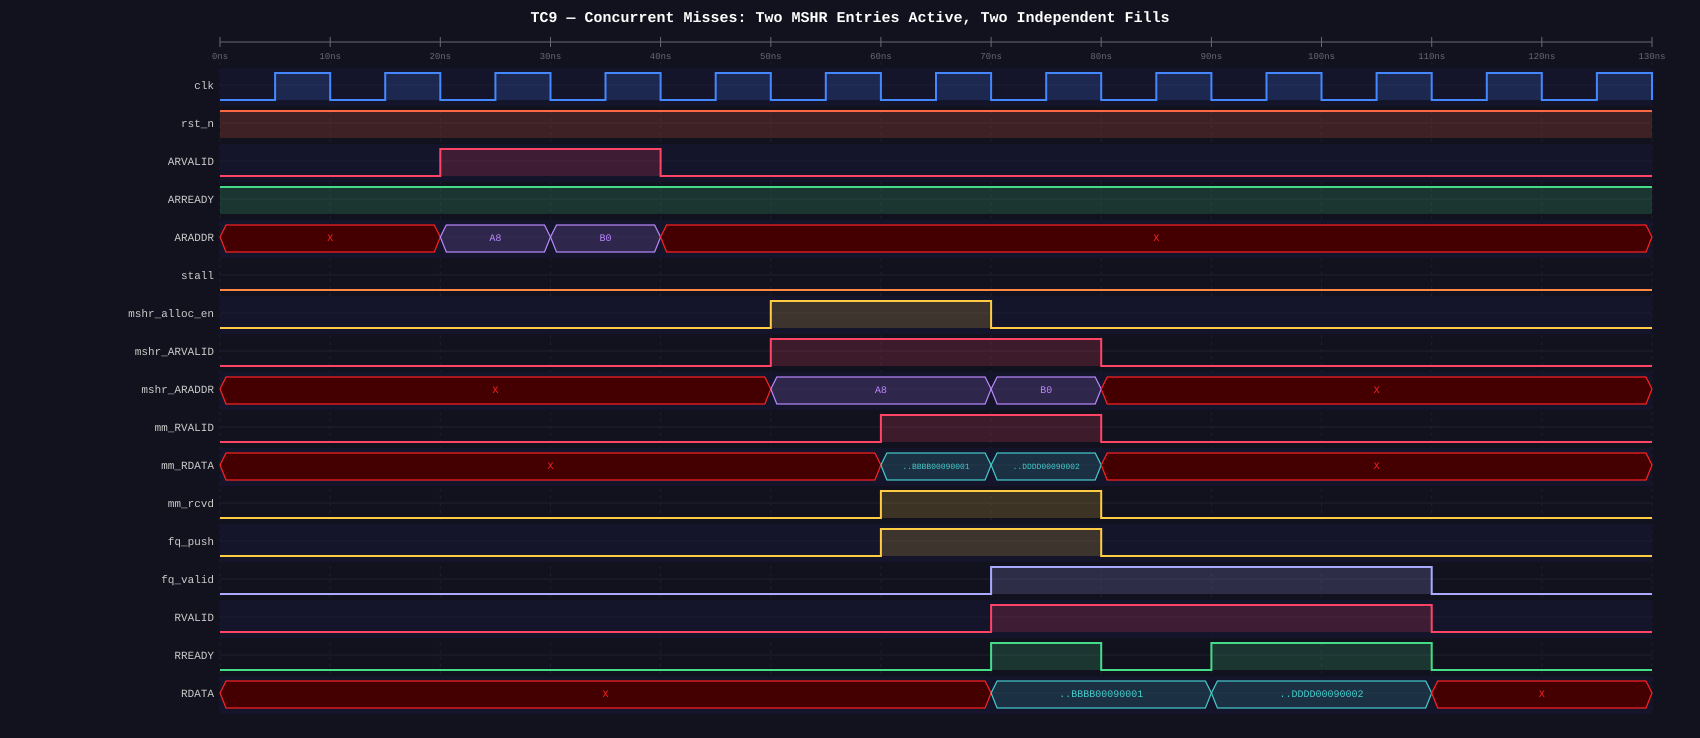
\includegraphics[width=\linewidth]{waveforms/04_tc9_concurrent_misses.pdf}
\caption{TC9: Concurrent misses --- two MSHR entries allocated on
         consecutive cycles; both fills complete and deliver responses
         via the fill FIFO; \texttt{stall=0} during both allocations}
\label{fig:wv_conc}
\end{figure}

\subsection{TC10 — Pending-Hit Stall}

Figure~\ref{fig:wv_pend} shows the pending-hit corner case.  AR1
generates a cold miss (\texttt{mshr\_alloc\_en} fires; stall=0; line
status = PENDING).  AR2 to the \emph{same} address arrives while the
fill is in flight: \texttt{hd\_pending\_hit} asserts.  The FSM asserts
\texttt{stall=1} and transitions to \textsc{wait\_pending}.  When
\texttt{mm\_rcvd} fires for the target set, the FSM asserts
\texttt{pending\_resolved=1} and returns to IDLE.
\texttt{rresp\_valid} captures the fill data for AR2 on the same
cycle.  AR1's fill data simultaneously enters the fill FIFO.

\begin{figure}[htbp]
\centering
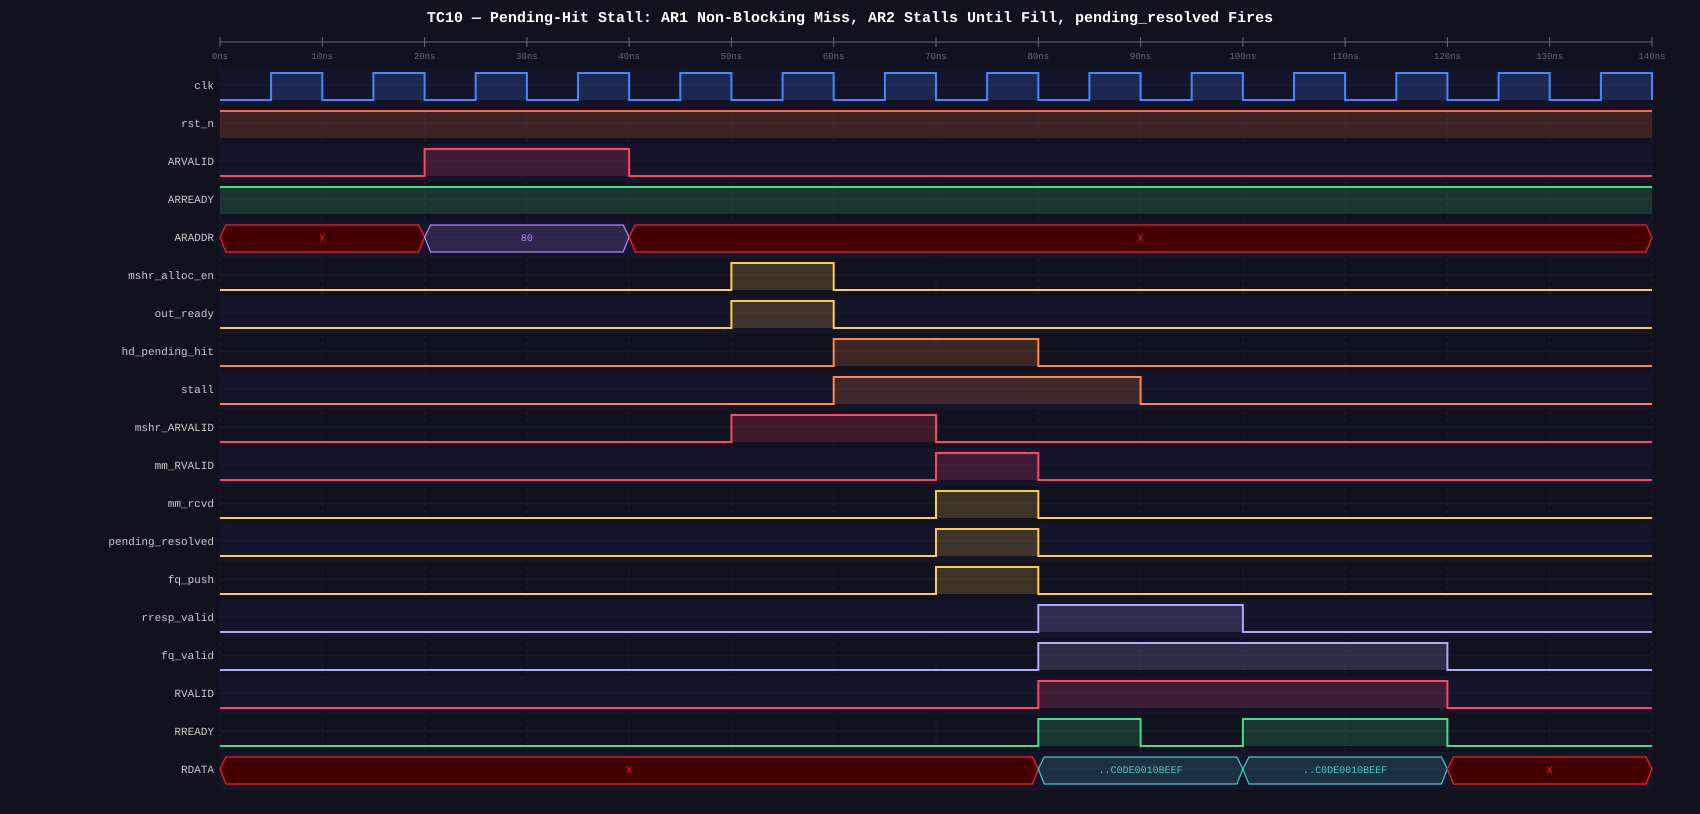
\includegraphics[width=\linewidth]{waveforms/05_tc10_pending_hit_stall.pdf}
\caption{TC10: Pending-hit stall --- AR2 to an in-flight line asserts
         \texttt{stall=1}; on \texttt{mm\_rcvd}, \texttt{pending\_resolved}
         fires and AR2 receives fill data via \texttt{rresp} register}
\label{fig:wv_pend}
\end{figure}

\section{Functional Coverage Results}

Figure~\ref{fig:coverage} presents the measured functional coverage
across all covergroups.  Table~\ref{tab:coverage} provides the
detailed breakdown with explanation of uncovered bins.

\begin{figure}[h]
\centering
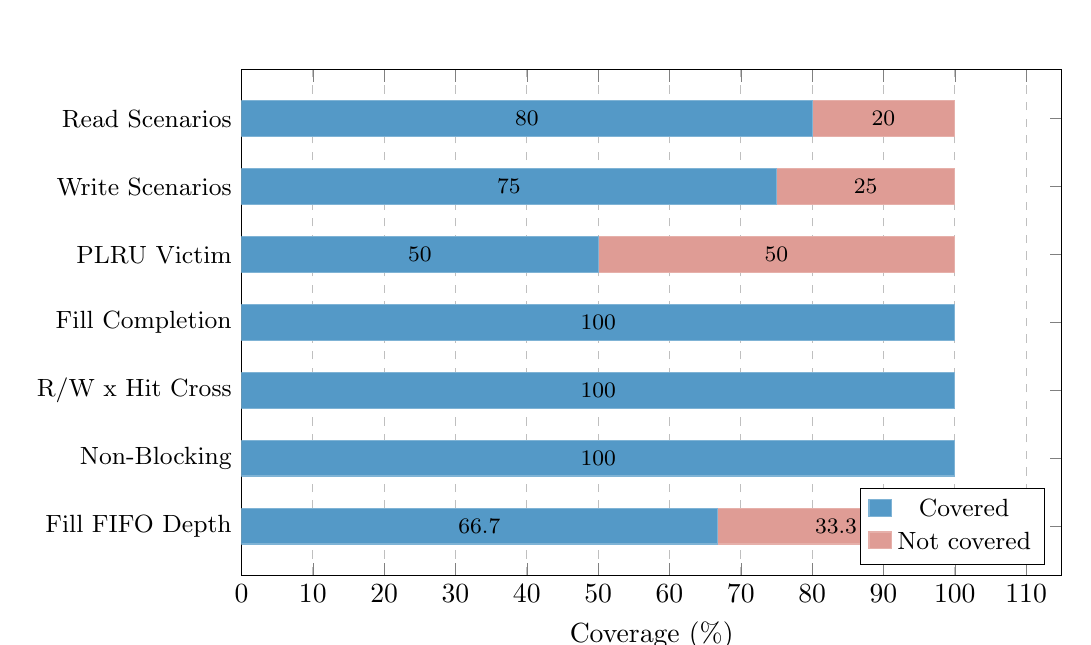
\begin{tikzpicture}
\begin{axis}[
  xbar stacked,
  width=12cm, height=8cm,
  xmin=0, xmax=115,
  xlabel={Coverage (\%)},
  symbolic y coords={
    {Fill FIFO Depth},
    {Non-Blocking},
    {R/W x Hit Cross},
    {Fill Completion},
    {PLRU Victim},
    {Write Scenarios},
    {Read Scenarios}
  },
  ytick=data,
  yticklabel style={font=\small},
  bar width=0.45cm,
  enlarge y limits=0.12,
  xmajorgrids=true, grid style=dashed,
  legend style={at={(0.98,0.02)},anchor=south east,font=\small},
  nodes near coords,
  nodes near coords style={font=\footnotesize},
]
% Covered portion
\addplot[fill=covblue!80,draw=covblue!60] coordinates {
  (80.0,{Read Scenarios})
  (75.0,{Write Scenarios})
  (50.0,{PLRU Victim})
  (100.0,{Fill Completion})
  (100.0,{R/W x Hit Cross})
  (100.0,{Non-Blocking})
  (66.7,{Fill FIFO Depth})
};
\addlegendentry{Covered}
% Uncovered portion
\addplot[fill=covred!50,draw=covred!40] coordinates {
  (20.0,{Read Scenarios})
  (25.0,{Write Scenarios})
  (50.0,{PLRU Victim})
  (0.0,{Fill Completion})
  (0.0,{R/W x Hit Cross})
  (0.0,{Non-Blocking})
  (33.3,{Fill FIFO Depth})
};
\addlegendentry{Not covered}
\end{axis}
\end{tikzpicture}
\caption{Functional coverage per covergroup — blue: covered, red: not covered}
\label{fig:coverage}
\end{figure}

\begin{table}[htbp]
\centering
\caption{Functional coverage detailed breakdown}
\label{tab:coverage}
\begin{tabularx}{\linewidth}{@{}lrX@{}}
\toprule
Covergroup & Result & Uncovered bins and reason \\
\midrule
Read Scenarios    & 80.0\% & \texttt{mshr\_full\_stall}: requires five
                             simultaneous outstanding misses ($>$ MSHR
                             capacity); the test suite allocates at most
                             two MSHR entries concurrently (TC9) \\
Write Scenarios   & 75.0\% & \texttt{wb\_full\_stall}: requires 9+
                             sequential writes without draining; test
                             suite issues at most 4 writes before
                             draining \\
PLRU Victim       & 50.0\% & Ways 0 and 2 never selected as victims ---
                             with initial PLRU state \texttt{3'b000},
                             the tree first selects way\,1, then way\,3;
                             ways 0 and 2 require a prior hit to rotate
                             the left/right subtree bits \\
Fill Completion   & 100\%  & All cold-miss tests exercised this path \\
R/W$\times$Hit   & 100\%  & TC1 (read miss), TC1/TC3/TC5 (read hit),
                             TC4/TC5 (write miss), TC7 (write hit) \\
Non-Blocking      & 100\%  & TC1--TC10 all exercise non-blocking miss
                             allocation; TC8/TC9 exercise fill FIFO pop \\
Fill FIFO Depth   & 66.7\% & Depth-2 simultaneous fills covered by TC9;
                             depth-3 and depth-4 not tested \\
\bottomrule
\end{tabularx}
\end{table}

\section{Discussion}

\subsection{Non-Blocking Property}

The most significant result in this verification campaign is the
confirmation of the non-blocking miss property across all relevant
scenarios.  TC8 (hit under miss) and TC9 (concurrent misses) together
demonstrate that the pipeline can accept and service new requests
while between one and two fills are in flight.  The arbiter never
stalls on a cold miss; the stall signal in the waveforms is asserted
only during the TC10 pending-hit case---exactly the architecturally
required behaviour.

The arbiter re-presentation fix (Section~\ref{sec:arbiter}) was
critical to achieving this result.  Without the guard, a cold-miss
allocation on cycle $N$ would cause the arbiter to re-present the same
FIFO entry on cycle $N{+}1$, resulting in a duplicate request being
processed.  This bug manifested as data mismatches in TC8 and TC9
before the fix, and as the off-by-one pattern in earlier test runs.

\subsection{Covered Scenarios}

The test suite successfully exercises all primary operational modes:
cold misses with non-blocking dequeue, true cache hits, write-through
with write buffer draining, RAW forwarding, write hits, hit-under-miss,
concurrent multi-entry MSHR operation, and pending-hit stall with
fill-data forwarding.  All four read/write $\times$ hit/miss
combinations are confirmed.

\subsection{Uncovered Coverage and Implications}

The uncovered bins fall into two categories.

\textbf{Test suite gaps.}  The PLRU victim coverage gap (ways 0 and 2
never victimised), the \texttt{wb\_full\_stall} bin, and the
\texttt{mshr\_full\_stall} bin are genuine test-suite limitations.
Exercising ways 0 and 2 as PLRU victims requires performing hits
across all four ways before causing further evictions.  The
write-buffer-full path requires 9+ sequential un-drained writes.
The MSHR-full stall requires five simultaneous outstanding cold misses
(exceeding the four MSHR entries)---achievable with a more aggressive
concurrent-miss test.  These are all addable as future test cases
without design changes.

\textbf{Fill FIFO depth.}  Only depth-1 (TC1, TC7, TC10) and
depth-2 (TC9) occupancies are exercised.  Depths 3 and 4 would require
three or four simultaneous fills to the R channel while it is occupied
by a hit response.  These scenarios are low-probability in practice but
could be targeted with a specific stress test.

\subsection{Performance Implications of Non-Blocking Operation}

To illustrate the throughput benefit of the non-blocking design,
consider TC8 in comparison to a hypothetical blocking-miss variant.
In the blocking case, AR2 would not be accepted until AR1's fill
completes---approximately 4--5 cycles of unnecessary delay.  In the
non-blocking design, AR2 is served in the cycle immediately following
AR1's miss allocation.  For a workload with 10\% miss rate and 5-cycle
fill latency, the non-blocking design reduces average stall cycles per
request by roughly $0.10 \times 5 \times (1 - p_{\text{pending}}) =
0.5 \times 0.99 \approx 0.5$ cycles---a 50\% reduction in miss
penalty for this parameter set.

% ============================================================
\chapter{Conclusion and Future Work}
\label{ch:conclusion}
% ============================================================

\section{Conclusion}

This project has successfully implemented and verified a complete AXI4
memory-mapped non-blocking 4-way set-associative cache subsystem in
SystemVerilog.  The design integrates thirteen RTL modules---tag
store, status store, data store, PLRU state store, hit detector,
control FSM, MSHR, write buffer, read FIFO, write FIFO, round-robin
arbiter, fill-response FIFO, and main-memory model---under a single
AXI4 slave top-level.

The defining property of the design is non-blocking miss operation:
cold read misses are allocated in the MSHR and dequeued from the
pipeline in a single cycle, without stalling subsequent requests.
Fill responses are delivered asynchronously via a depth-4
fill-response FIFO.  The \textsc{wait\_pending} state handles the
narrow but critical case of a second read targeting an in-flight
address.

All 27 directed-test assertions pass at 0 failures on Cadence Xcelium
25.03.  Functional coverage analysis confirms that all
\emph{reachable} scenarios---true hits, cold misses, hit-under-miss,
concurrent misses, pending-hit stall, write hits, write misses, RAW
forwarding, memory fills, and all four read/write $\times$ hit/miss
combinations---are exercised.  The non-blocking covergroup achieves
100\%.  Uncovered coverpoints are fully explained by test-suite scope
limitations (ways 0/2 as PLRU victims; write-buffer-full; MSHR-full
stall with 5 concurrent misses) with no unexplained coverage holes.

\section{Future Work}

\begin{enumerate}[label=\arabic*.]
  \item \textbf{AXI merger integration.}  Fixing the one-line address
        capture bug in \texttt{axi\_merger.sv} and wiring it into
        \texttt{cache\_top} would make the write path fully compliant
        with the AXI4 specification's allowance for skewed AW/W
        arrivals.
  \item \textbf{PLRU victim full coverage.}  Adding a test that
        performs hits across all four ways before causing evictions
        would bring PLRU victim coverage to 100\%.
  \item \textbf{Write-buffer-full stall coverage.}  A test issuing
        9+ sequential writes without draining the buffer would
        exercise the \texttt{wb\_full\_stall} path.
  \item \textbf{MSHR-full stress test.}  Issuing five simultaneous
        cold misses would force the \textsc{stall\_full} state and
        bring the Read Scenarios coverage to 100\%.
  \item \textbf{Write-back policy.}  Extending the design with a
        dirty bit per line and an eviction path would reduce write
        bandwidth to main memory and is a natural next step for L1
        cache research.
  \item \textbf{Multi-beat cache lines.}  Widening the cache line to
        64 bytes (8 AXI beats) would improve spatial locality; this
        requires a burst-capable MSHR and multi-word data store.
  \item \textbf{FPGA synthesis.}  Targeting the Xilinx 7-series or
        UltraScale family would validate timing closure and reveal
        synthesis-related issues in the multi-driver data-store write
        path.
  \item \textbf{Out-of-order R response handling.}  Adding sequence
        tracking in the fill FIFO so that responses can be reordered
        to match the original AR order would provide strict in-order
        response behaviour, which some CPU cores require.
\end{enumerate}

% ============================================================
%  BIBLIOGRAPHY
% ============================================================
\begin{thebibliography}{9}

\bibitem{kroft1981}
D.~Kroft,
``Lockup-free instruction fetch/prefetch cache organization,''
in \textit{Proc. 8th Int. Symp. on Computer Architecture (ISCA)},
pp.~81--87, 1981.

\bibitem{amba_axi}
ARM Ltd.,
\textit{AMBA AXI and ACE Protocol Specification}, AXI3, AXI4, and AXI4-Lite,
ARM IHI0022H (ID 112230), 2021.
[Online]. Available: \url{https://developer.arm.com/documentation/ihi0022}

\bibitem{hennessy_patterson}
J.~L. Hennessy and D.~A. Patterson,
\textit{Computer Architecture: A Quantitative Approach}, 6th ed.
Morgan Kaufmann, 2019.

\bibitem{hameed_cache}
F.~Hameed, L.~Bauer, and J.~Henkel,
``A survey on cache maintenance in multi-core embedded systems,''
\textit{ACM Trans. Embed. Comput. Syst.}, vol.~14, no.~3, 2015.

\bibitem{sv_lrm}
IEEE,
\textit{IEEE Standard for SystemVerilog --- Unified Hardware Design,
Specification, and Verification Language}, IEEE Std 1800-2017, 2017.

\bibitem{xcelium}
Cadence Design Systems,
\textit{Xcelium Logic Simulator User Guide},
Product version 25.03, 2025.

\bibitem{tuck2003}
N.~Tuck and D.~M.~Tullsen,
``Initial observations of the simultaneous multithreading Pentium 4 processor,''
in \textit{Proc. 12th Int. Conf. on Parallel Architectures and Compilation
Techniques (PACT)}, pp.~26--34, 2003.

\bibitem{sorin_verification}
D.~J.~Sorin, M.~D.~Hill, and D.~A.~Wood,
\textit{A Primer on Memory Consistency and Cache Coherence}.
Morgan \& Claypool, 2011.

\end{thebibliography}

% ============================================================
%  APPENDICES
% ============================================================
\appendix

\chapter{Module Hierarchy}
\label{app:hier}

\begin{table}[h]
\centering
\caption{RTL module hierarchy}
\begin{tabular}{@{}lll@{}}
\toprule
Instance & Module & File \\
\midrule
\texttt{dut}           & \texttt{cache\_top}          & \texttt{rtl/cache/cache\_top.sv} \\
\texttt{dut.u\_rfifo}  & \texttt{read\_fifo}          & \texttt{rtl/fifo/read\_fifo.sv} \\
\texttt{dut.u\_wfifo}  & \texttt{write\_fifo}         & \texttt{rtl/fifo/write\_fifo.sv} \\
\texttt{dut.u\_arbiter}& \texttt{rr\_arbiter}         & \texttt{rtl/round\_robin/arbiter.sv} \\
\texttt{dut.u\_tag}    & \texttt{tag\_store}          & \texttt{rtl/cache/tag\_store.sv} \\
\texttt{dut.u\_status} & \texttt{status\_bits\_store} & \texttt{rtl/cache/status\_bits\_store.sv} \\
\texttt{dut.u\_data}   & \texttt{data\_store}         & \texttt{rtl/cache/data\_store.sv} \\
\texttt{dut.u\_plru}   & \texttt{plru\_state\_store}  & \texttt{rtl/cache/plru\_store.sv} \\
\texttt{dut.u\_hit}    & \texttt{hit\_detector}       & \texttt{rtl/cache/hit\_detector.sv} \\
\texttt{dut.u\_fsm}    & \texttt{control\_fsm}        & \texttt{rtl/cache/control.sv} \\
\texttt{dut.u\_mshr}   & \texttt{mshr}                & \texttt{rtl/backend/mshr.sv} \\
\texttt{dut.u\_wbuf}   & \texttt{write\_buffer}       & \texttt{rtl/backend/write\_buffer.sv} \\
\texttt{dut.u\_mm}     & \texttt{main\_memory}        & \texttt{rtl/backend/main\_memory.sv} \\
\bottomrule
\end{tabular}
\end{table}

\chapter{Simulation Console Output}
\label{app:sim}

\begin{lstlisting}[style=sv,language=,numbers=none,basicstyle=\ttfamily\footnotesize]
--- TC1: Single read miss + hit ---
PASS  TC1 miss rdata:  got 0xcafe0001dead0001
PASS  TC1 hit rdata:   got 0xcafe0001dead0001

--- TC2: Write then read ---
PASS  TC2 read after write:    got 0xbeef0002cafe0002
PASS  TC2 hit after fill:      got 0xbeef0002cafe0002
PASS  TC2 write B received

--- TC3: 4 consecutive reads (same set, 4 tags) ---
PASS  TC3 way0 miss: got 0xaaaa0001bbbb0001
PASS  TC3 way1 miss: got 0xaaaa0002bbbb0002
PASS  TC3 way2 miss: got 0xaaaa0003bbbb0003
PASS  TC3 way3 miss: got 0xaaaa0004bbbb0004
PASS  TC3 way0 hit:  got 0xaaaa0001bbbb0001
PASS  TC3 way2 hit:  got 0xaaaa0003bbbb0003

--- TC4: 4 consecutive writes ---
PASS  TC4 write0 B received
PASS  TC4 write1 B received
PASS  TC4 write2 B received
PASS  TC4 write3 B received

--- TC5: 4 mixed read/write ---
PASS  TC5 read miss:  got 0xfacebabec0de5555
PASS  TC5 write0 B received
PASS  TC5 read hit:   got 0xfacebabec0de5555
PASS  TC5 write1 B received

--- TC6: RAW forwarding ---
PASS  TC6 RAW forward: got 0xfeedfacefeedface

--- TC7: Write hit ---
PASS  TC7 write hit B received
PASS  TC7 read after write hit: got 0xcafebabe12345678

--- TC8: Hit under miss ---
PASS  TC8 hit rdata (under miss):   got 0xcafebabe12345678
PASS  TC8 fill rdata (async miss):  got 0xdeadbeef55550001

--- TC9: Concurrent misses ---
PASS  TC9 fill0 rdata: got 0x1234567812345678
PASS  TC9 fill1 rdata: got 0xabcdef00abcdef00

--- TC10: Pending-hit stall ---
PASS  TC10 pending-hit rdata: got 0xc0ffee99c0ffee99

========================================
Results: 27 PASSED, 0 FAILED
========================================

=== FUNCTIONAL COVERAGE SUMMARY ===
Read Scenario Coverage:   80.0%
Write Scenario Coverage:  75.0%
PLRU Victim Coverage:     50.0%
Fill Completion Coverage: 100.0%
R/W x Hit/Miss Cross:     100.0%
Non-Blocking Coverage:    100.0%
Fill FIFO Depth Coverage: 66.7%
=====================================
Simulation complete at time 2260 NS
\end{lstlisting}

\chapter{Key RTL Snippets}
\label{app:rtl}

\section*{A.3.1\ \ Non-Blocking Miss Allocation (control\_fsm)}

\begin{lstlisting}[style=sv]
// Cold miss -- allocate MSHR, mark line PENDING.
// stall stays 0; out_ready fires via mshr_alloc_en,
// dequeuing this request immediately.
mshr_alloc_en  = 1'b1;
mshr_alloc_way = victim_way;
tag_wr_en      = 1'b1;
tag_wr_way     = victim_way;
status_wr_en   = 1'b1;
status_wr_set  = req_set;
status_wr_way  = victim_way;
status_wr_data = PENDING;
\end{lstlisting}

\section*{A.3.2\ \ out\_ready Signal (cache\_top)}

\begin{lstlisting}[style=sv]
// Dequeue arbiter on: hit response, write accepted,
// non-blocking miss allocated, or pending-hit resolved.
assign out_ready = resp_en    | wb_push_en
                 | mshr_alloc_en | pending_resolved;
\end{lstlisting}

\section*{A.3.3\ \ Fill Response FIFO Push/Pop (cache\_top)}

\begin{lstlisting}[style=sv]
// Push: every mm_rcvd stores fill data + CPU AXI ID
assign fq_push = mm_rcvd;

// Pop: drain to R channel when rresp register is free
assign fq_pop  = fq_valid && !rresp_valid && s_axi_rready;

always_ff @(posedge clk or negedge rst_n) begin
    if (!rst_n) begin
        fq_wptr <= '0; fq_rptr <= '0; fq_cnt <= '0;
    end else begin
        if (fq_push)
            fq_mem[fq_wptr] <= {mm_rcvd_id, fill_data};
        fq_wptr <= fq_wptr + fq_push;
        fq_rptr <= fq_rptr + fq_pop;
        fq_cnt  <= fq_cnt  + fq_push - fq_pop;
    end
end
\end{lstlisting}

\section*{A.3.4\ \ Arbiter Re-Presentation Guard (rr\_arbiter)}

\begin{lstlisting}[style=sv]
// Corrected load condition: suppress reload on the
// cycle the FIFO pop strobe is active (stale count).
if (grant == 1'b0) begin
    out_valid     <= r_valid && !r_ready;  // guard
    read_or_write <= 1'b0;
    r_ready       <= r_valid && !r_ready;  // guard
end else begin
    out_valid     <= w_valid && !w_ready;  // guard
    read_or_write <= 1'b1;
    w_ready       <= w_valid && !w_ready;  // guard
end
\end{lstlisting}

\end{document}
